%%% -*-LaTeX-*-

\chapter{Whole-Program Trace Analysis}
We present a tool called
DiffTrace that approaches debugging via {\em whole program} tracing and
diffing of typical and erroneous traces.
%
After collecting these traces,
a user-configurable front-end filters out irrelevant function calls
and then summarizes loops in the retained function
calls based on state-of-the-art loop extraction algorithms.
%
Information about these loops is inserted
into concept lattices, which we use to
compute salient dissimilarities to narrow down bugs.
%
DiffTrace is a clean start that addresses
debugging features missing in existing approaches.
%
Our experiments on an MPI/OpenMP program called
ILCS and initial measurements on LULESH, a DOE miniapp,
demonstrate the advantages of the proposed debugging approach.

\section{Introduction}
\label{sec:ch3_intro}
Debugging high-performance computing code
remains a challenge at all levels of scale.
%
Conventional HPC debuggers~\cite{ddt,totalview}
excel at many tasks such as examining the execution
state of a complex simulation in detail
and allowing the developer to re-execute
the program close to the point of failure.
%
However, they do not provide a good understanding
of why a program version that worked earlier
failed upon upgrade or feature addition.
%
Innovative solutions are needed to highlight the
salient differences between two executions in a manner
that makes debugging easier as well as more systematic.
%
A recent study conducted under the auspices of the
DOE~\cite{hpcdoe}
provides a comprehensive survey
of existing debugging tools.
%
It classifies them under
four software organizations (serial, multithreaded,
multi-process, and hybrid), six
method types (formal methods, static analysis, dynamic
analysis, nondeterminism control, anomaly detection,
and parallel debugging), and lists a total of 30 specific
tools.
%
Despite this abundance of activity and tools, many
significant problems remain to be solved before debugging
{\em can be approached by the HPC community as a collaborative
activity} so that HPC developers can extend a common
framework.


Almost all debugging approaches seek to find outliers (``unexpected
executions'') amongst thousands of running processes and threads.
%
The approach taken by most existing tools is to
look for symptoms in a specific bug-class that they cover.
%
Unfortunately,
this approach calls for a programmer having a good guess of what
the underlying problem might be,
and to then pick the right set of tools to deploy.
%
If the guess is wrong, the programmer has no choice but to
refine their guess
and look for bugs in another class,
re-executing the application and hoping for
better luck with another tool.
%
This iterative loop of re-execution followed by applying a
best-guess tool for the suspected bug class can potentially consume
large amounts of execution cycles and wastes an
expert developer's time.
%
More glaring is the fact that these tools must recreate the
execution traces yet again: they do not have means to hand off
these traces to another tool or cooperate in symbiotic ways.



We cannot collect all relevant pieces of information
necessary to detect all possible bug classes such as
resource leaks, deadlocks, and data races.
%
Each such bug requires its attributes to be kept.
%
Also, debugging is not fully automatable (it is
an undecidable problem in general) and must involve human thinking:
at least to reconcile what is observed against the deeper application-level semantics.
%
However, (1)~we believe that it is still possible to collect one standard set
of data and use it to make an initial triage in such
a way that it can guide a later, deeper debugging phase to locate
which of the finer bug gradations (e.g., resource leaks or races) brought
the application down.
%
Also, (2)~we believe that it is possible to engage the human {\em with respect
to understanding structured presentations of information}.



Our DiffTrace framework addresses both issues.
%
The common set of data it uses is a {\em whole program
function call trace} collected per process/thread.
%
DiffTrace relies on
novel ways to diff a normal trace and a fault-laden trace to guide the
debugging engineer closer to the bug.
%
While our work has not (yet) addressed situations in
which millions of threads and thousands of processes run
for days before they produce an error,
we strongly believe that we can get there
once we understand the pros and cons of our initial
implementation of the DiffTrace tool, which is described in this paper.
%
The second issue is handled in DiffTrace by offering a novel
collection of modalities for understanding program execution diffs.
%
We now elaborate on these points by addressing the following three problems.



\subsection{Problem 1 -- Collecting Whole-Program Heterogeneous Function-Call Traces
Efficiently\/} Not only must we have the ability
to record function calls and returns at one
API such as MPI, increasingly we must collect calls/returns at multiple
interfaces (e.g., OpenMP, PThreads, and even inner levels such as TCP).
%
The growing use of heterogeneous parallelization necessitates that we
understand MPI and OpenMP activities (for example) to locate cross-API
bugs that are often missed by other tools.
%
Sometimes, these APIs contain the actual error (as opposed to the user code), and it would be attractive to have this debugging ability.


{\em Solution to Problem 1:\/}
In DiffTrace, we choose Pin-based whole program binary tracing, with
tracing filters that allow the designer to collect a suitable mixture of API
calls/returns.
%
We realize this facility using
ParLOT, a tool designed by us and published earlier~\cite{parlot}.
%
In our research, we have thus far demonstrated the advantage of
ParLOT with respect to collecting both MPI and OpenMP traces
from a {\em single run of a hybrid MPI/OpenMP program}.
%
We demonstrate that, from this single type of trace, it is possible
to pick out MPI-level bugs and/or OpenMP-level bugs.
%
While whole-program tracing
may sound extremely computation and storage intensive, ParLOT employs
lightweight on-the-fly compression techniques to keep these overheads low.
%
It achieves compression ratios exceeding 21,000~\cite{parlot},
thus making this approach practical, demanding
only a few kilobytes per second per core of bandwidth.


\subsection{Problem 2 -- Need to Generalize Techniques for Outlier Detection\/}
Given that outlier detection is central to debugging,
it is essential to use efficient representations of the traces
to be able to systematically compute
{\em distances} between them without
involving human reasoning.
%
The representation must also be versatile enough to
be able to ``diff'' the traces
with respect to {\em an extensible number of vantage points}.
%
These vantage points could be diffing traces concerning process-level activities,
thread-level activities, a combination thereof,
or even finite sequences of process/thread calls (say, to locate {\em changes}
in caller/callee relationships).


{\em Solution to Problem 2:\/}
DiffTrace employs {\em concept lattices} to amalgamate the collected traces.
%
Concept lattices have previously been employed in HPC to perform structural
clustering of process behaviors~\cite{weberStructural} to present performance data more
meaningfully to users.
%
The authors of that paper use the notion of {\em Jaccard distances}
to cluster performance results that are closely related to process structures
(determined based on caller/callee relationships).
%
In DiffTrace, we employ incremental algorithms for building and maintaining
concept lattices from the ParLOT-collected traces.
%
In addition to Jaccard distances, in our work, we also perform hierarchical
clustering of traces and provide a tunable threshold for outlier detection.
%
We believe that these uses of concept lattices and refinement approaches
for outlier detection are new in HPC debugging.


\subsection{Problem 3 -- Loop Summarization\/}
Most programs spend most of their time in loops.
%
Therefore, it is important to employ state-of-the-art algorithms for
loop extraction from execution traces.
%
It is also important
to be able to diff two executions with respect to changes in their looping behaviors.
%
In our experience, presenting such changes using good visual metaphors
tends to highlight many bug types immediately.


{\em Solution to Problem 3:\/}
DiffTrace utilizes the rigorous notion of Nested Loop Representations (NLRs) for
summarizing traces and representing loops.
%
Each repetitive loop structure is given an identifier, and nested loops are
expressed as repetitions of this identifier exponentiated (as with regular
expressions).
%
This approach to summarizing loops can help manifest
bugs where the program does not hang or crash but nevertheless
runs differently in a manner that informs the developer engaged in debugging.

{\bf Organization\/}:
%
\S\ref{sec:ch3_overview} illustrates the contributions of this paper on a simple example.
%
\S\ref{sec:ch3_algo} presents the algorithms underlying DiffTrace in more detail.
%
\S\ref{sec:ch3_ilcs-case-study} summaries the experimental methodology before showing a medium-sized case study involving MPI and OpenMP.
%
\S\ref{sec:ch3_lulesh} shows initial measurements and examples on LULESH~\cite{LULESH2:changes}, a DOE common mini app.
%
\S\ref{sec:ch3_related} summarizes selected related works.
%
\S\ref{sec:ch3_discussion} concludes the paper with a discussion.

%
% \Noindent To summarize, the key contributions of this paper are the following
% \begin{itemize}
% \item A method to organize function call traces collected from processes and
%       threads into concept lattices, and a method to
%       detect loops from dynamic traces (Section~\ref{sec3}).
%
% \item Details of the algorithms employed in DiffTrace (Section~\ref{sec4}).
%
% \item Experimental studies on a heterogeneous program called
%       Iterated Local Champion Search (ILCS, Section~\ref{sec5}).
%
% \item Strengths and limitations of DiffTrace, plans for future work (Section~\ref{sec6}).
% \end{itemize}
%

 

\section{DiffTrace Overview}
\label{sec:ch3_overview}
\subsection{High-level Overview}

\begin{figure}[t]
\caption{DiffTrace Overview}
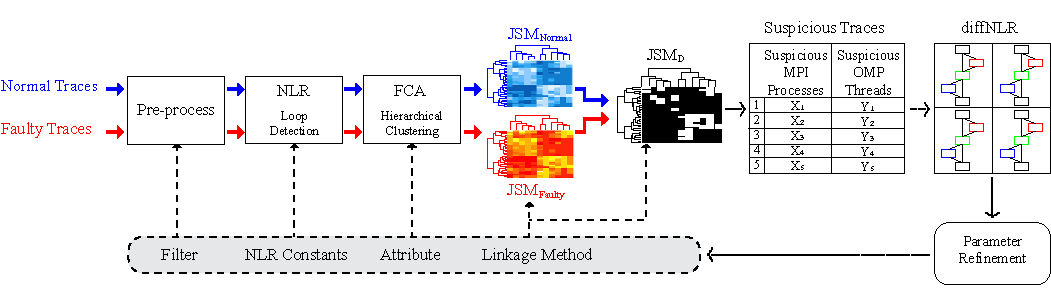
\includegraphics[width=1\textwidth]{diffTrace/figs/overview4.pdf}
%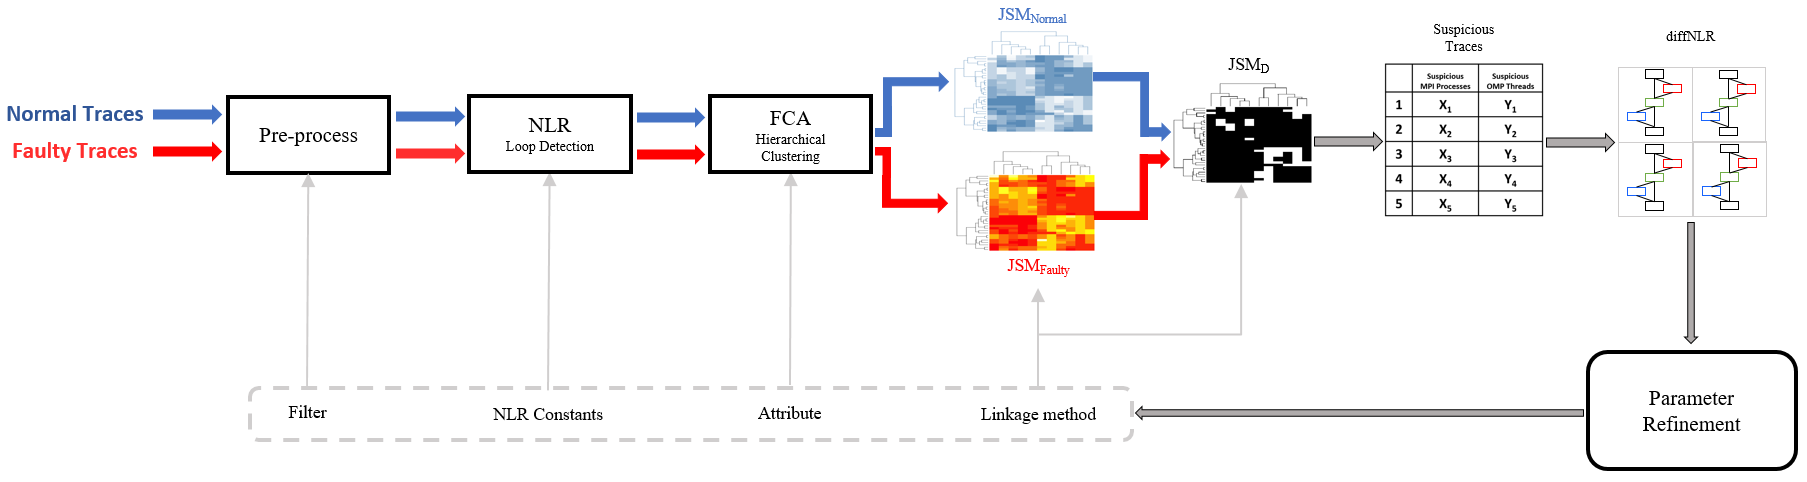
\includegraphics[]{figs/overview.png}
%\includegraphics[]{figs/overv}
\label{fig.diffTraceOverview}
\end{figure}

DiffTrace employs ParLOT's whole-program function-call and return trace-collection mechanism, where ParLOT captures traces via Pin~\cite{pin} and incrementally compresses them using a new compression scheme~\cite{parlot}.
%
ParLOT can capture functions at two levels:
the \textit{main image} (which does not include library code)
and \textit{all images} (including all library code).
%
As the application runs,
ParLOT generates per-thread trace files that
contain the compressed sequence of the IDs of the executed functions.
%
The compression mechanism is light-weight yet effective,
thus reducing not only the required bandwidth and storage but also the
runtime relative to not compressing the traces.
As a result, ParLOT can capture whole-program traces at low overhead
while leaving most of the disk bandwidth to the application.
%
Using whole-program traces substantially reduces the number of overall
debug iterations because it allows us to repeatedly analyze the
traces offline with different filters.


Figure \ref{fig.diffTraceOverview} provides an overview
of the DiffTrace toolchain
in terms of the blue flows (fault-free) and red flows
(faulty).
%
In a broad sense,
code-level faults in HPC applications (e.g.,
the use of wrong subscripts) turn into observable code-level
misbehaviors
(e.g., an unexpected number of loop iterations), many of which
turn into application-level issues.
%
In our study of DiffTrace, we evaluate
success merely in terms of the efficacy of observing
these misbehaviors in response to injected code-level
faults (we rely on a rudimentary fault injection framework
complemented by manual fault injection).

The preprocessing stage removes calls/returns at the ignored APIs.
%
The nested loop recognition (NLR)
mechanism then extracts loops from traces.
The resulting information not only
serves as a lossless abstraction to
ease the rest of the trace analysis but also
serves as a {\em per-thread measure of progress}.
%
The FCA (Formal Concept Analysis) stage conducts a systematic way to arrange objects (in our case threads)
and attributes (we support a rich collection of attributes
including the set of function calls a thread makes, the
set of {\em pairs} of function calls made---this reflects calling
context---etc.).
%
Weber et al.'s work~\cite{weberStructural,clbook} employs FCA exactly in
this manner (including the use of pairs of calls),
however, for grouping performance information.
%
Our new contribution is showing that FCA can play a central
role in debugging HPC applications.


While faults induce asymmetries (``aberrations'') in program behaviors,
one cannot locate faults merely by locating the asymmetries in
an overall collection of process traces.
%
The reason is that even in a collection of MPI processes or threads within
these processes, some processes/threads may serve as a master while others
serve as workers.
%
Thus, we must have a base level of similarities computed even for normal
behaviors and then compute how {\em this similarity relation changes} when
faults are introduced.
%
This is highlighted by
the blue and red rectangular patches in
Figure~\ref{fig.diffTraceOverview} that, respectively,
iconify the {\em Jaccard similarity
  matrices} computed for the normal behavior (above) and
the erroneous behavior (below).
%
This is shown as
the ``diff Jaccard similarity matrix'' in greyscale at the
juncture of JSM$_{normal}$ and JSM$_{faulty}$.


After the JSM$_{D}$ matrix is computed, we
invoke a hierarchical clustering algorithm that computes the ``B-score''
and helps rank suspicious traces/processes.
%
The diffNLR representation is then extracted.
%
Intuitively, this is a diff of the loop structures of the normal and abnormal
threads/processes.
%
This diagram shows (as with git diff and text diff) a {\em main stem} comprised of green rectangles
(``common looping structure'') and red/blue {\em diff rectangles} showing how the loop structures of
the normal and erroneous threads differ with respect to the main stem.
%
We show that this presentation often helps the debugging engineer
locate the faults.


Last but not least,
we strongly believe that a framework such as DiffTrace can
serve as an important HPC community resource.
%
Each debugging tool designer who uses DiffTrace can extend
it by incorporating new attributes and clustering methods, but
otherwise retain the overall tool structure.
%
Such a ``playground'' for developing and exploring new methods for
debugging does not exist in HPC.
%
There is also the intriguing possibility that
many of the 30-odd tools mentioned in \S\ref{sec:ch4_intro}
{\em can be made to focus on the problems highlighted
  by diffNLR}, thus gaining efficiency (this will be part of our future work).


In this paper, we describe DiffTrace as a
{\em relative debugging}~\cite{relative-debugging}
tool, in that bugs are caught with respect
to JSM$_{D}$ which is a {\em change} from
the previous code version found working.
%
However, many types of faults may be apparent
just by analyzing JSM$_{faulty}$: for instance,
processes whose execution got truncated
will look highly dissimilar to those that
terminated normally.
%
In those use cases of DiffTrace,
the B-score based ranking can then be made
on JSM$_{faulty}$ directly.

%---






\subsection{Example Walk-through}

We now employ
Figure~\ref{fig.oddEven}---a textbook MPI odd/even sorting example---to
illustrate DiffTrace.
%
Odd/even sorting is a parallel variant
of bubble sort
and operates in two alternating phases:
in the \textit{even phase}, the even processes exchange (conditionally swap)
values with their right neighbors, and in the \textit{odd phase},
the odd processes exchange values with their right neighbors.
%
%The for loop in line 4 of \texttt{oddEvenSort()} iterates over the phases of the algorithm. Based on the phase, the appropriate partner for each rank is computed by the function \texttt{findPtr()} (line 6). The odd/even ranks then exchange their chunks of data (lines 9-13) and sort, merge, and copy operations are performed on the received data (denoted by \texttt{...} in line 15 for simplicity).


\begin{figure}[b]
\centering
\caption{Simplified MPI implementation of Odd/Even Sort}
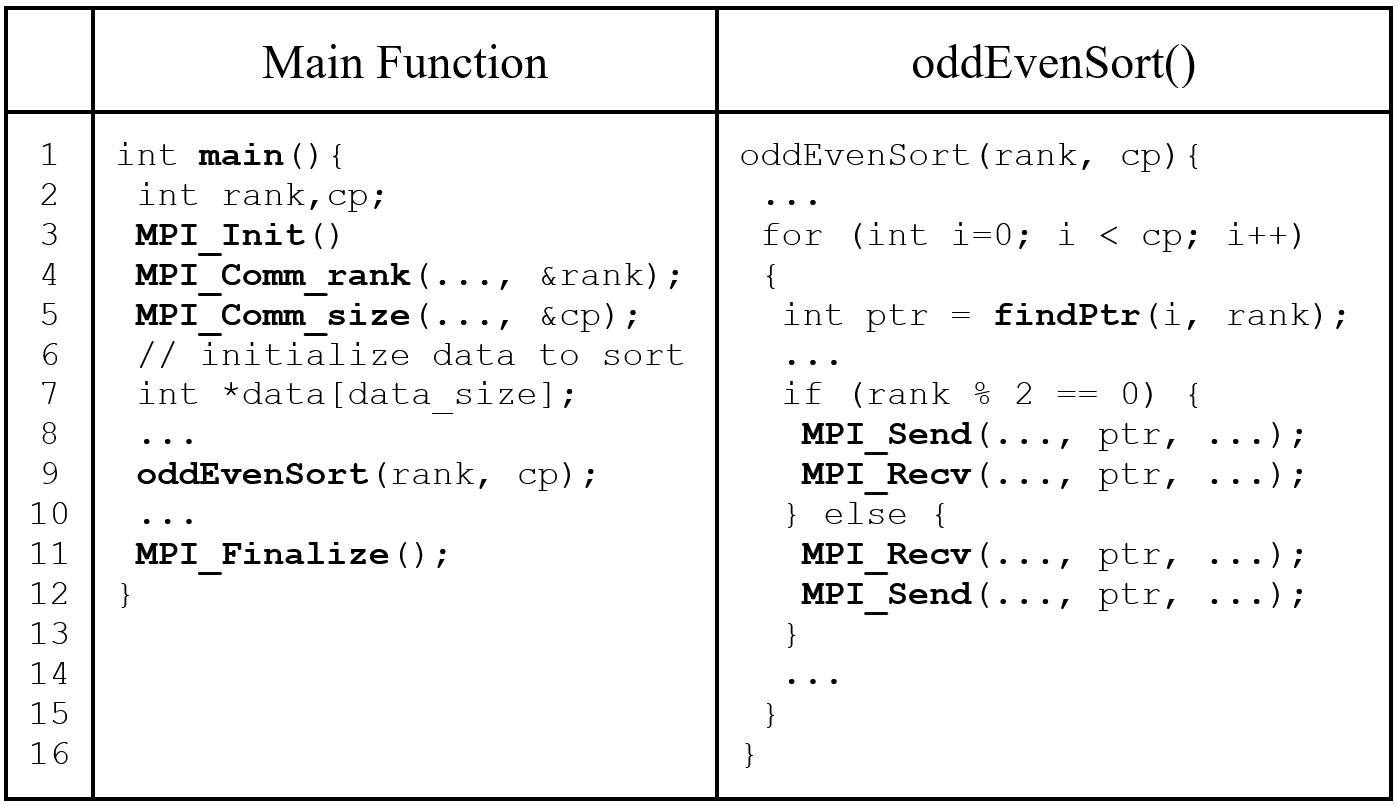
\includegraphics[width=.8\textwidth]{diffTrace/figs/oddEven.png}
\label{fig.oddEven}
\end{figure}

A waiting trap in this example is this: the user may have
swapped the {\tt Recv; Send} order in the {\tt else} part,
creating head-to-head {\tt ``Send || Send''} deadlock
under low-buffering (MPI EAGER limit).
%
We will now show how DiffTrace helps pick out this root-cause.

\subsection{Pre-processing}
% Please add the following required packages to your document preamble:
% \usepackage{multirow}
\begin{table}[]
\centering
\caption{Predefined filters}
\label{tab:filters}
\scalebox{0.72}{
\begin{tabular}{|c|c|l|}
\hline
\textbf{Category} & \textbf{Sub-Category} & \multicolumn{1}{c|}{\textbf{Description}} \\ \hline
\multirow{2}{*}{Primary} & Returns & Filter out all returns \\ \cline{2-3}
 & PLT & \begin{tabular}[c]{@{}l@{}}Filter out the ".plt" function calls for external functions/procedures that \\ their address needs to be resolved dynamically from Procedure Linkage \\ Table (PLT)\end{tabular} \\ \hline
\multirow{4}{*}{MPI} & MPI All & Only keep functions that start with "MPI\_" \\ \cline{2-3}
 & MPI Collectives & Only keep MPI collective calls (MPI\_Barrier, MPI\_Allreduce, etc) \\ \cline{2-3}
 & MPI Send/Recv & Only keep MPI\_Send, MPI\_Isend, MPI\_Recv, MPI\_Irecv and MPI\_Wait \\ \cline{2-3}
 & MPI Internal Library & Keep all inner MPI library calls \\ \hline
\multirow{3}{*}{OMP} & OMP All & Only keep OMP calls (starting with GOMP\_) \\ \cline{2-3}
 & OMP Critical & Only keep OMP\_CRITICAL\_START and OMP\_CRITICAL\_END \\ \cline{2-3}
 & OMP Mutex & Only keep OMP\_Mutex calls \\ \hline
\multirow{4}{*}{System} & Memory & Keep any memory related functions (memcpy, memchk, alloc, malloc, etc) \\ \cline{2-3}
 & Network & Keep any network related functions (network, tcp, sched, etc) \\ \cline{2-3}
 & Poll & Keep any poll related functions (poll, yield, sched, etc) \\ \cline{2-3}
 & String & Keep any string related functions (strlen, strcpy, etc) \\ \hline
\multirow{2}{*}{Advanced} & Custom & Any regular expression can be captured \\ \cline{2-3}
 & Everything & Does not filter anything \\ \hline
\end{tabular}}
\end{table}

Using ParLOT's decoder, each trace is first decompressed.
Next, the desired functions are extracted based on predefined
(Table \ref{tab:filters}) or custom regular expressions
(i.e., \textit{filters}) and kept for later phases.
%All other trace information is discarded.
%
Table \ref{tab:oddEvenPT} shows the pre-processed traces ($T_i$) of odd/even sort with four processes.
$T_i$ is the trace that stores the function calls of process $i$.

\begin{table}[]
\centering
\caption{The generated traces for odd/even execution with four processes}
\label{tab:oddEvenPT}
\scalebox{0.75}{
\begin{tabular}{|l|l|l|l|}
\hline
\rowcolor[HTML]{EFEFEF}
\multicolumn{1}{|c|}{\cellcolor[HTML]{EFEFEF}\textbf{$T_0$}} & \multicolumn{1}{c|}{\cellcolor[HTML]{EFEFEF}\textbf{$T_1$}} & \multicolumn{1}{c|}{\cellcolor[HTML]{EFEFEF}\textbf{$T_2$}} & \multicolumn{1}{c|}{\cellcolor[HTML]{EFEFEF}\textbf{$T_3$}} \\ \hline
... & ... & ... & ... \\ \\[-1em]  \hline
main & main & main & main \\ \\[-1em]  \hline
MPI\_Init & MPI\_Init & MPI\_Init & MPI\_Init \\ \\[-1em]  \hline
MPI\_Comm\_Rank & MPI\_Comm\_Rank & MPI\_Comm\_Rank & MPI\_Comm\_Rank \\ \\[-1em]  \hline
MPI\_Comm\_Size & MPI\_Comm\_Size & MPI\_Comm\_Size & MPI\_Comm\_Size \\ \\[-1em]  \hline
... & ... & ... & ... \\ \\[-1em]  \hline
oddEvenSort & oddEvenSort & oddEvenSort & oddEvenSort \\ \\[-1em]  \hline
... & ... & ... & ... \\ \\[-1em] \hline
findPtr & findPtr & findPtr & findPtr \\ \hline
\rowcolor[HTML]{FFCCC9}
{\color[HTML]{333333} MPI\_Send} & \cellcolor[HTML]{CBCEFB}{\color[HTML]{333333} MPI\_Recv} & {\color[HTML]{333333} MPI\_Send} & \cellcolor[HTML]{CBCEFB}{\color[HTML]{333333} MPI\_Recv} \\ \hline
\rowcolor[HTML]{FFCCC9}
{\color[HTML]{333333} MPI\_Recv} & \cellcolor[HTML]{CBCEFB}{\color[HTML]{333333} MPI\_Send} & {\color[HTML]{333333} MPI\_Recv} & \cellcolor[HTML]{CBCEFB}{\color[HTML]{333333} MPI\_Send} \\ \hline
... & ... & ... & ... \\ \hline
findPtr & findPtr & findPtr & findPtr \\ \hline
\rowcolor[HTML]{FFCCC9}
{\color[HTML]{333333} MPI\_Send} & \cellcolor[HTML]{CBCEFB}{\color[HTML]{333333} MPI\_Recv} & {\color[HTML]{333333} MPI\_Send} & \cellcolor[HTML]{CBCEFB}{\color[HTML]{333333} MPI\_Recv} \\ \hline
\rowcolor[HTML]{FFCCC9}
{\color[HTML]{333333} MPI\_Recv} & \cellcolor[HTML]{CBCEFB}{\color[HTML]{333333} MPI\_Send} & {\color[HTML]{333333} MPI\_Recv} & \cellcolor[HTML]{CBCEFB}{\color[HTML]{333333} MPI\_Send} \\ \hline
... & ... & ... & ... \\ \hline
MPI\_Finalize & MPI\_Finalize & MPI\_Finalize & MPI\_Finalize \\ \hline
\end{tabular}}
\end{table}






\subsection{Nested Loop Representation}

Virtually all dynamic statements are found within loops.
%
Function calls within a loop body yield \textit{repetitive patterns}
in ParLOT traces.
%
Inspired by ideas for the detection of repetitive patterns in strings \cite{nakamura_fast_2013}
and other data structures \cite{kmr},
we have adapted the Nested Loop Recognition (NLR) algorithm by Ketterlin et al.~\cite{Ketterlin-nlr}
to detect repetitive patterns in ParLOT traces (cf.~Section \ref{subsec:algo-nlr}).
Detecting such patterns can be used to measure the progress of each thread,
revealing unfinished or broken loops that may be the consequence of a fault.



\begin{table}[]
\centering
\caption{NLR of traces}
\label{tab:oddEvenPT-NLR}
\scalebox{0.75}{
\begin{tabular}{|l|l|l|l|}
\hline
\rowcolor[HTML]{EFEFEF}
\multicolumn{1}{|c|}{\cellcolor[HTML]{EFEFEF}\textbf{$T_0$}} & \multicolumn{1}{c|}{\cellcolor[HTML]{EFEFEF}\textbf{$T_1$}} & \multicolumn{1}{c|}{\cellcolor[HTML]{EFEFEF}\textbf{$T_2$}} & \multicolumn{1}{c|}{\cellcolor[HTML]{EFEFEF}\textbf{$T_3$}} \\ \hline
MPI\_Init & MPI\_Init & MPI\_Init & MPI\_Init \\ \\[-1em]  \hline
MPI\_Comm\_Rank & MPI\_Comm\_Rank & MPI\_Comm\_Rank & MPI\_Comm\_Rank \\ \\[-1em]  \hline
MPI\_Comm\_Size & MPI\_Comm\_Size & MPI\_Comm\_Size & MPI\_Comm\_Size \\ \\[-1em]  \hline
\rowcolor[HTML]{FFCCC9}
{\color[HTML]{333333} L0 \^{} 2} & \cellcolor[HTML]{CBCEFB}{\color[HTML]{333333} L1 \^{} 4} & {\color[HTML]{333333} L0 \^{} 4} & \cellcolor[HTML]{CBCEFB}{\color[HTML]{333333} L1 \^{} 2} \\ \hline
MPI\_Finalize & MPI\_Finalize & MPI\_Finalize & MPI\_Finalize \\ \hline
\end{tabular}}
\end{table}



For example, the loop in line 3 of \texttt{oddEvenSort()} (Figure \ref{fig.oddEven}) iterates
four times when run with four processes.
Thus each $T_i$ contains four occurrences of either [\texttt{MPI\_Send}-\texttt{MPI\_Recv}] (even $i$)
or [\texttt{MPI\_Recv}-\texttt{MPI\_Send}] (odd $i$).
By keeping only MPI functions and converting each $T_i$ into its equivalent NLR,
Table \ref{tab:oddEvenPT} can be reduced to Table \ref{tab:oddEvenPT-NLR} where \textbf{L0} and \textbf{L1}
represent the \textit{loop body} [\texttt{MPI\_Send}-\texttt{MPI\_Recv}] and
[\texttt{MPI\_Recv}-\texttt{MPI\_Send}], respectively.
The integer after the \^{} symbol in NLR represents the \textit{loop iteration count}.
Note that, since the first and last processes only have one-way communication with their neighbors,
$T_0$ and $T_3$ perform only half as many iterations.

\begin{table}[]
\caption{Formal Context of odd/even sort example}
\label{tab:sampleContext}
\scalebox{0.7}{
\begin{tabular}{l|cccccc}
 & \multicolumn{1}{l}{MPI\_Init()} & \multicolumn{1}{l}{MPI\_Comm\_Size()} & \multicolumn{1}{l}{MPI\_Comm\_Rank()} & \multicolumn{1}{l}{L0} & \multicolumn{1}{l}{L1} & \multicolumn{1}{l}{MPI\_Finalize()} \\ \hline
Trace 0 & $\times$ & $\times$ & $\times$ & $\times$ &  & $\times$ \\
Trace 1 & $\times$ & $\times$ & $\times$ &  & $\times$ & $\times$ \\
Trace 2 & $\times$ & $\times$ & $\times$ & $\times$ &  & $\times$ \\
Trace 3 & $\times$ & $\times$ & $\times$ &  & $\times$ & $\times$
\end{tabular}}
\end{table}

\subsection{Hierarchical Clustering via FCA}
Processes in HPC applications are known to fall into predictable equivalence classes.
%
The widely used and highly successful STAT tool~\cite{stat} owes most of its
success for being able to efficiently collect stack traces (nested sequences of function
calls), organize them as prefix-trees, and equivalence the processes into teams that
evolve in different ways.
%
Coalesced stack trace graphs (CSTG, \cite{cstg}) have proven effective in
locating bugs within Uintah~\cite{uintah} and perform stat-like equivalence class formation,
albeit with the added detail of maintaining calling contexts.
%
Inspired by these ideas, FCA-based clustering provides the next logical level of refinement
in the sense that (1)~we can pick any of the multiple attributes one can mine from traces (e.g.,
pairs of function calls, memory regions accessed by processes, locks held by threads, etc.), and (2)~form this equivalencing relation quite naturally by computing the Jaccard distance between processes/threads.
%
In general,
such a classification is powerful enough to
distinguish structurally different threads from one another
(e.g., MPI processes from OpenMP threads in hybrid MPI+OpenMP applications)
and reduce the search space for bug location to a few representative classes of traces that
are distinctly dissimilar.\footnote{As emphasized earlier, we perform ``sky subtraction'' as
  in astronomy to locate comets; in our case, we diff the diffs, which is
  captured in JSM$_{D}$.}

A \textit{formal context} is a triple $K = (G, M, I)$
where $G$ is a set of \textbf{objects},
$M$ is a set of \textbf{attributes},
and $I \subseteq G \times M$ is an incidence relation that expresses
\textit{which objects have which attributes}.
Table \ref{tab:sampleContext} shows the formal context of the preprocessed odd/even-sort traces.
%
We can employ as attributes either the function calls themselves or the detected loop bodies
(each detected loop is assigned a unique ID, and one can diff with respect to these IDs).
%
The context shows that all traces include the functions MPI\_Init(),
MPI\_Comm\_size(), MPI\_Comm\_rank() and MPI\_Finalize().
The even traces contain the loop \textit{L0} and the odd traces the loop \textit{L1}.
%

% \hl{Definition of formal concept (needed?) figure }\ref{fig:formalConceptDefinition} :
%
% \begin{figure}[]
% \centering
% \caption{Formal Concept Definition}
% 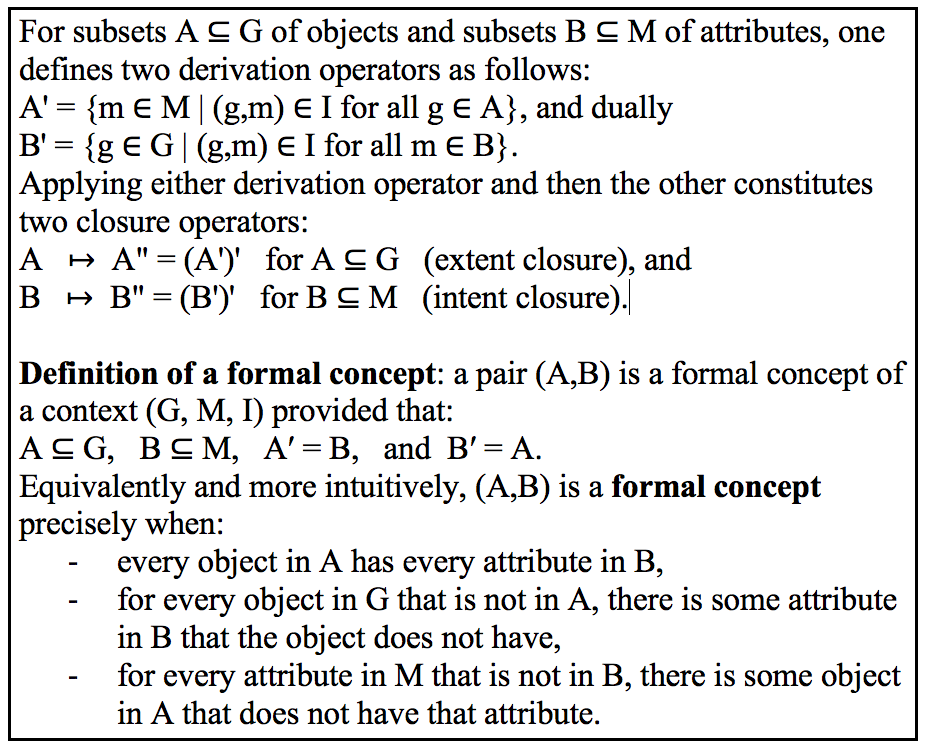
\includegraphics[width=0.45\textwidth]{figs/formalConceptDefinition.png}
% \label{fig:formalConceptDefinition}
% \end{figure}

%A \textit{concept lattice} can be derived from a \textit{formal context} by specifying \textit{formal concepts}
%(Figure \ref{fig:formalConceptDefinition})
%and a \textit{partial order} on them.
%Concept lattices are represented as a directed acyclic graph where concepts are nodes and the
%order on them determines the edges.
%
Figure \ref{fig:sampleCL} shows the concept lattice derived from the formal context in
Table~\ref{tab:sampleContext} and is interpreted as follows:

\begin{compactitem}
\item The top node indicates that all traces share MPI\_Init(),
  MPI\_Comm\_size(), MPI\_Comm\_rank() and MPI\_Finalize().
    \item The bottom node signifies that none of the traces share all attributes.
    \item The middle nodes show that $T_0$ and $T_2$ are different from  $T_1$ and $T_3$.
\end{compactitem}



% Once the redundant labels are removed from the lattice, each object (trace) and attribute appears in the lattice exactly once. Consequently, the nodes of the lattice form the desired grouping, since it is guaranteed that each trace belongs to exactly one group. However, the concept lattice itself does not provide similarity values for the distinct groups of traces. The \textit{Jaccard Index}, also known as \textit{Intersection over Union}, measures the \textit{distance} between sets $A$ and $B$ in terms of the ratio of the \textit{intersection} size of $A$ and $B$ over the size of their \textit{union}.
%

%


\begin{figure}[t]
\centering
\begin{minipage}{.45\textwidth}
  \centering
  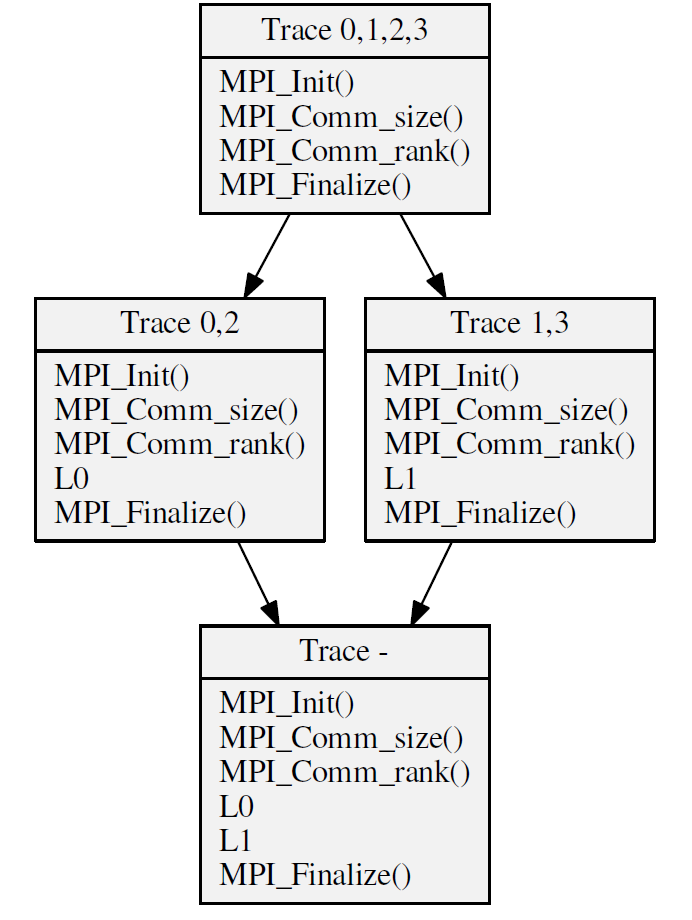
\includegraphics[width=.9\linewidth]{diffTrace/figs/sampleCL.png}
  \caption{Sample Concept Lattice from Object-Attribute Context in Table \ref{tab:sampleContext}}
  \label{fig:sampleCL}
\end{minipage}
\begin{minipage}{.45\textwidth}
\centering
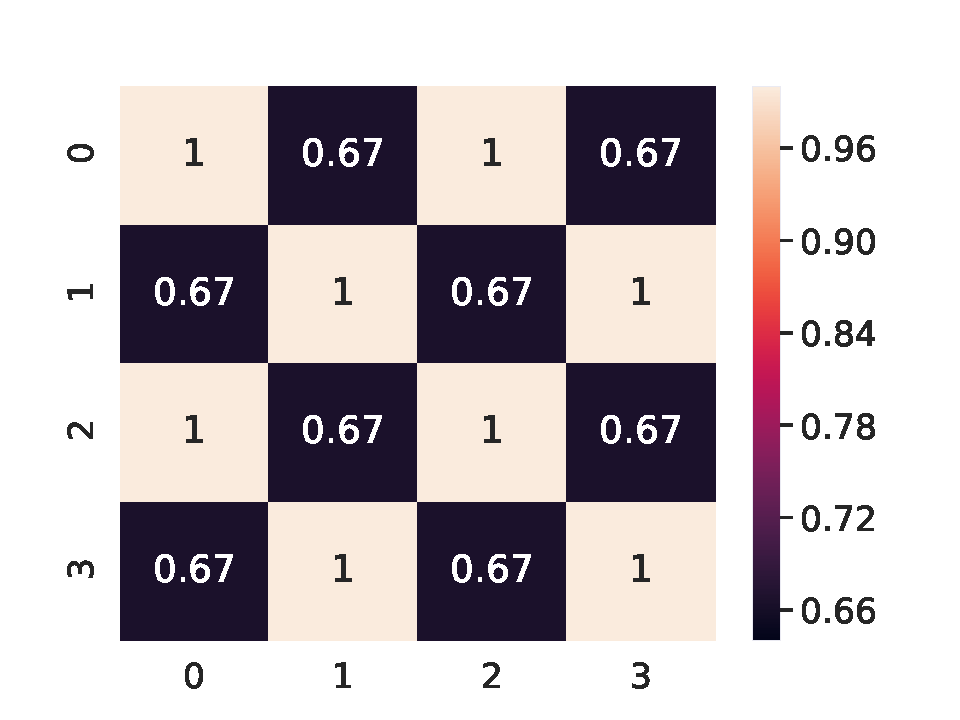
\includegraphics[width=.9\linewidth]{diffTrace/figs/oddEvenJSM2.pdf}
\caption{Pairwise Jaccard Similarity Matrix (JSM) of MPI Processes in Sample Code}
\label{fig:jsm2}
\end{minipage}

\end{figure}


%\begin{figure}[]
%\centering
%\scalebox{0.8}{
%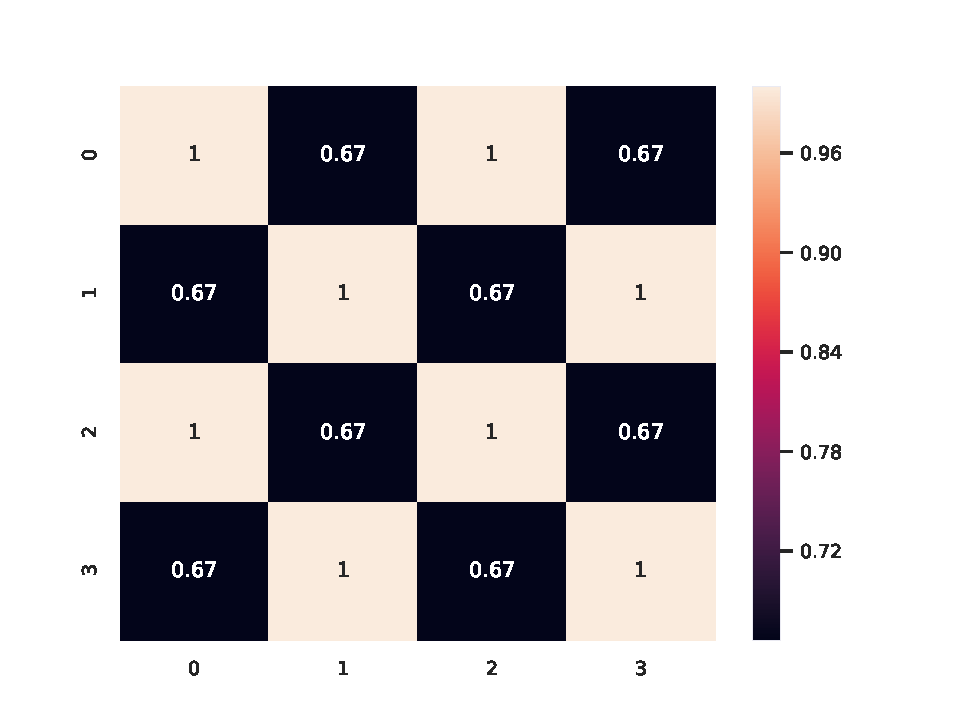
\includegraphics[width=3.4in]{figs/oddEvenJSM.pdf}}
%\caption{Pairwise Jaccard Similarity Matrix (JSM) of MPI processes in sample code}
%\label{fig:jsm}
%\end{figure}


% For any pair of $(T_i, T_j)$, the number of attributes in the Lowest Common Ancestor (LCA) node of $T_i$ and $T_j$ in the lattice is the number of attributes that $T_i$ and $T_j$ have in common (intersection). The sum of the number of attributes of the nodes on the path from each $T_i$ and $T_j$ to their LCA is the union. This property is one of the motivations for using concept lattices as classifier since it makes computing the union and intersection easy and fast.
%
% Some algorithms for extracting concepts from contexts and constructing the concept lattice require the whole context to be present in the memory.
%

The complete pairwise Jaccard Similarity Matrix (JSM) can easily be computed from concept lattices.
%
For large-scale executions with thousands of threads, it is imperative
to employ incremental algorithms to
construct concept lattices (detailed in Section \ref{subsec:algo-cl}).
%
% Through an incremental concept-lattice-construction approach,
% DiffTrace extracts attributes (\hl{table that shows attributes})
% from NLR traces and injects them into a concept lattice one trace at a time
%
Figure \ref{fig:jsm2}
shows the heatmap
% (explain this)
of the JSM obtained from the concept lattice in Figure \ref{fig:sampleCL}.
%
DiffTrace uses the JSM to form equivalence classes of traces by hierarchical clustering.
%
Next, we show how the differences between two hierarchical clusterings from two executions
(faulty vs.~normal) reveal which traces have been affected the most by the fault.


\subsection{Detecting Suspicious Traces via JSM$_{D}$}
% So far,
% we have explained how DiffTrace can narrow down the search space from numerous long traces to just a few equivalent JSMs (i.e., clusters).
% %
JSM$_{normal}$[i][j] (JSM$_{faulty}$[i][j]) shows the Jaccard similarity score of $T_i$ and $T_j$ from the normal trace ($T_i^\prime$ and $T_j^\prime$).
%
% However, we are interested in detecting what changed the most due to the fault.
% with respect to the ``natural asymmetry'' of the application.
%
%In other words, DiffTrace abstracts function call traces into JSMs, which are reflections of asymmetry among traces.
As explained earlier, we compute
JSM$_{D}$ to detect outlier executions, where
JSM$_{D}$ = $|$JSM$_{faulty} - $JSM$_{normal}|$.

%
We sort the suggestion table based on the \textit{B-score}
similarity metric of two hierarchical clusterings \cite{fowlkes83} (cf.~Section \ref{subsec:algo-bscore}).
%
A single iteration through the
DiffTrace loop
(with a single set of parameters shown as a dashed box in Figure \ref{fig.diffTraceOverview})
may still not detect the root-cause of a bug.
%
The user can then (1)~alter the linkage method employed in computing the hierarchical clustering
(reorder the dendrograms built to achieve the clustering),
(2)~alter the FCA attributes, (3)~adjust the NLR constants (loops are extracted with
realistic complexity by observing repetitive patterns inside a preallocated buffer),
and/or (4)~the front-end filters.
%
This is shown in the iterative loop in
Figure \ref{fig.diffTraceOverview}.

\subsection{Evaluation}

%The resulting outlier traces are candidates for the potential cause of the change in the program behavior and thus, a potential fault root cause or fault manifestation.
%

%
%Also, a different set of parameters might produce inaccurate suggestions (false positives).
%

\begin{figure}[t]
\begin{minipage}{.2\textwidth}
\centering
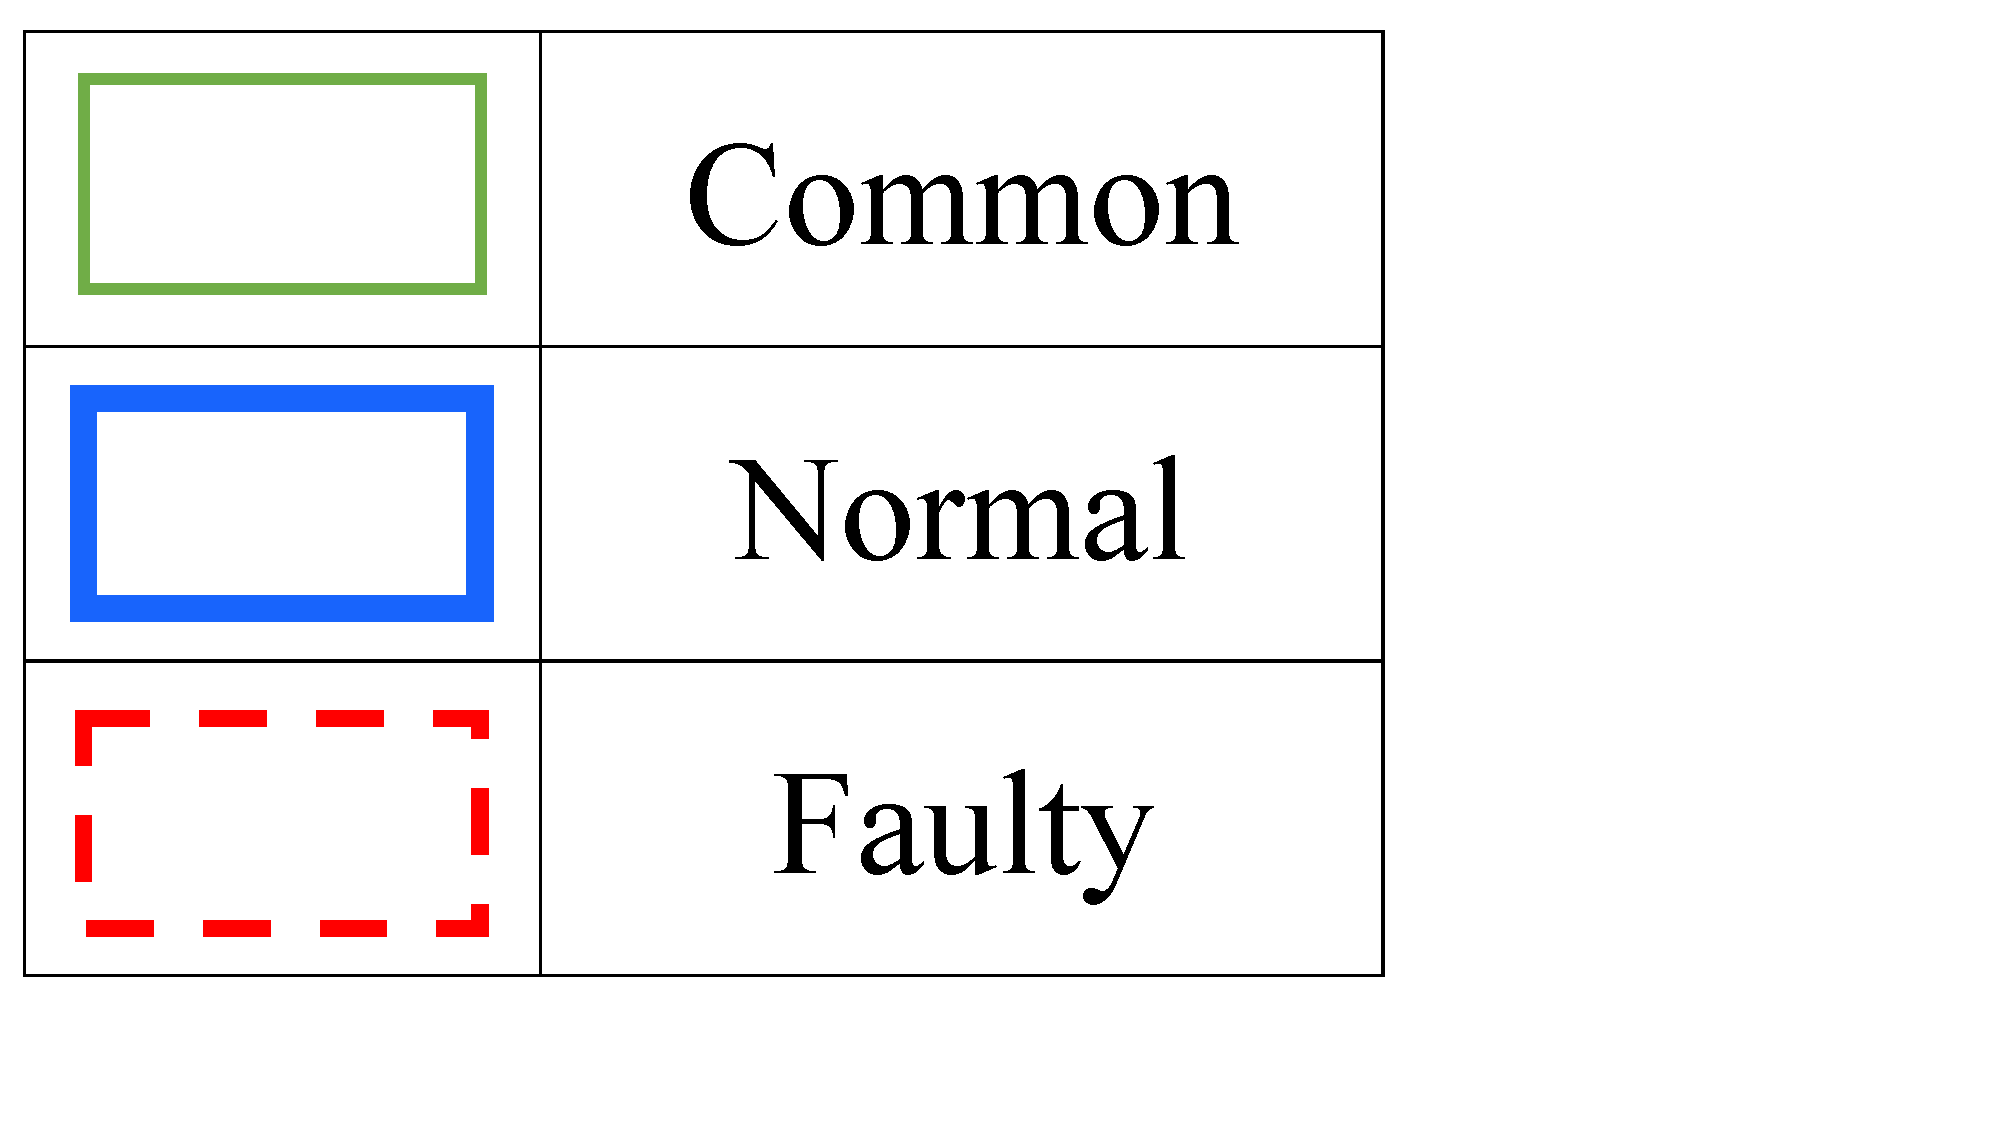
\includegraphics[width=\textwidth]{diffTrace/figs/legend.pdf}
\caption{Legend}
\label{fig:legend}
\end{minipage}
\begin{minipage}{.38\textwidth}
    \centering
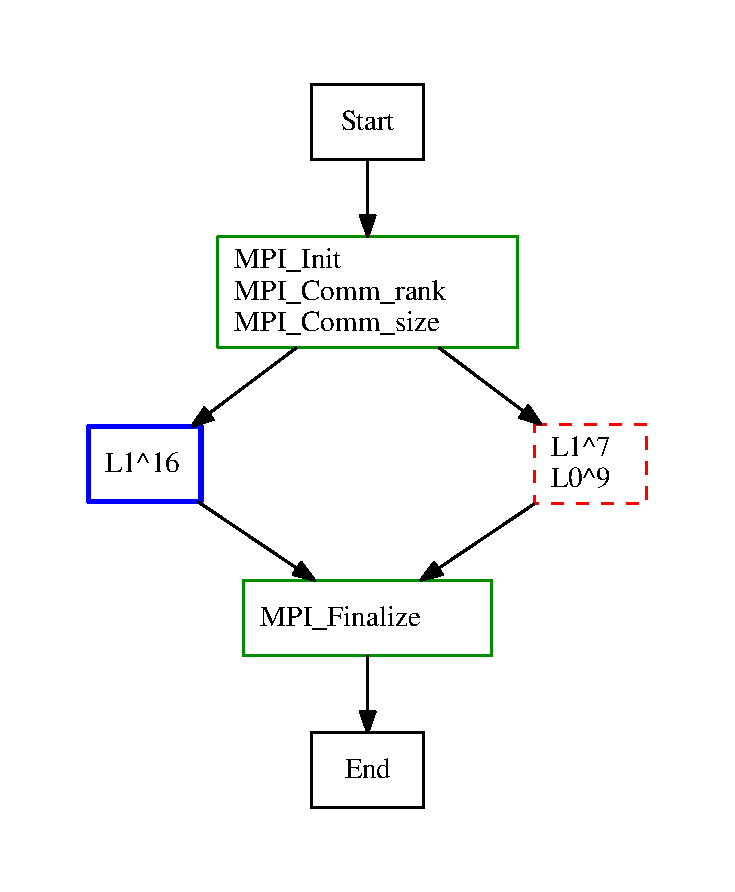
\includegraphics[width=\textwidth]{diffTrace/figs/b-11.mpi.0K10-5.pdf}
\caption{swapBug}
\label{fig:swapbug}
\end{minipage}
%\caption{diffNLR Example}
%\label{fig:sampleDiffNLR}
\begin{minipage}{.38\textwidth}
\centering
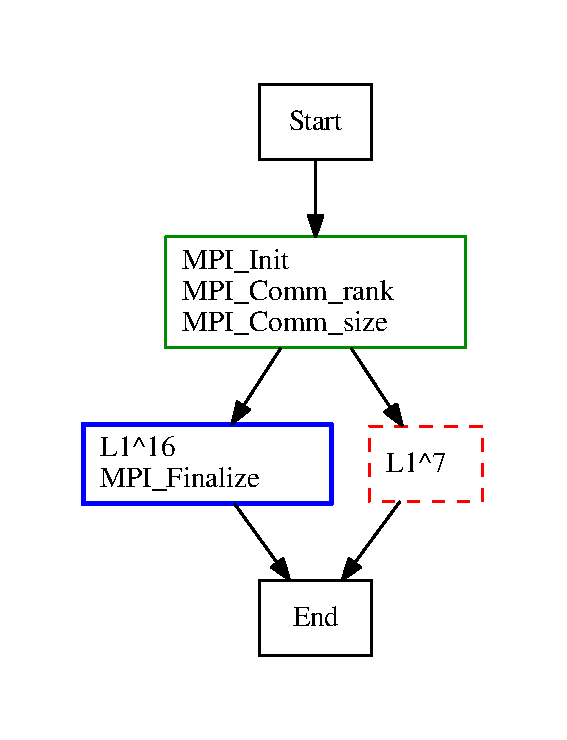
\includegraphics[width=0.9\linewidth]{diffTrace/figs/adl-11.mpi.0K10-5.pdf}
\caption{dlBug}
\label{fig:dlbug}
\end{minipage}
\end{figure}

To evaluate the effectiveness of DiffJSM, we planted two artificial bugs (\textit{swapBug}
and \textit{dlBug}) in the code from Figure \ref{fig.oddEven} and ran it with 16 processes.
%
\textit{swapBug} swaps the order of MPI\_Send and MPI\_Recv in rank 5
after the seventh iteration of the loop in line 3 of \texttt{oddEvenSort},
simulating a potential deadlock. \textit{dlBug} simulates an actual deadlock in the same location
(rank 5 after the seventh iteration).
%
Upon collection of ParLOT traces from the execution of the buggy code versions,
DiffTrace first decompresses them and filters out all non-MPI functions.
Then two major loops are detected, \textbf{L0} and \textbf{L1} (identical to the ones in Table \ref{tab:oddEvenPT-NLR}),
that are supposed to loop 16 times in the even and odd traces,
respectively (except for the first and last traces, which loop just eight times).

After constructing concept lattices and their corresponding JSMs, trace 5 appears as the trace that got
affected the most by the bugs because row 5 (showing the similarity score of $T_5$ relative to all other traces)
(JSM$_{normal}$[5][i] for $i \in [0,16)$)
  changed the most after the bug was introduced.
  %Consequently, it means that $T^\prime_5$ affected the asymmetry of all $T_i$s.
%
The differences between the suggested suspicious trace ($T^\prime_s$)
and its corresponding normal trace ($T_s$) is visualized by \textit{diffNLR}.


\subsubsection{diffNLR}
To highlight the differences in an easy-to-understand manner, DiffTrace visually separates the common and different blocks of a pair of pre-processed traces via \textit{diffNLR}, a graphical visualization of the \texttt{diff} algorithm \cite{diff-myers}.
%






\texttt{diff} takes two sequences $S_A$ and $S_B$ and computes the minimal \textit{edit} to convert $S_A$ to $S_B$. This algorithm is used in the GNU \texttt{diff} utility to compare two text files and in git for efficiently keeping track of file changes.
Since ParLOT preserves the order of function calls, each trace $T_i$ is totally ordered. Thus \textit{diff} can expose the differences of a pair of $T$s. \textit{diffNLR} aligns common and different blocks of a pair of sequences (e.g., traces) horizontally and vertically, making it easier for the analyst to see the differences at a glance.
For simplicity, our implementation of \textit{gdiff} only takes one argument $x$ that denotes \textit{the suspicious trace}.

diffNLR$(x) \equiv $ diffNLR$(T_x,T_x^\prime)$
%
where $T_x$ is the trace of thread/process $x$ of a normal execution and $T^\prime_x$ is the corresponding trace of the faulty execution.

Figure \ref{fig:swapbug} shows the diffNLR(5) of \textit{swapBug} where $T_5$ iterates over the loop [MPI\_Recv - MPI\_Send] 16 times (L1\^{}16) after the MPI initialization while the order swap is well reflected in $T_5^\prime$ (L1\^{}7 - L0\^{}9). Both processes seem to terminate fine by executing MPI\_Finalize().
However, diffNLR(5) of \textit{dlBug} (Figure \ref{fig:dlbug}) shows that, while $T_5$ executed MPI\_Finalize, $T_5^\prime$ got stuck after executing L1 seven times and never reached MPI\_Finalize.

This example illustrates how our approach can locate the part of each execution that was impacted by a fault. Having an understanding of \textit{how the application should behave normally} can reduce the number of iterations by picking the right set of parameters sooner.


%\begin{figure}[]
%\centering
%\caption{A line change in oddEvenSort (left) that might cause a deadlock in oddEvenSort\_DL (right)}
%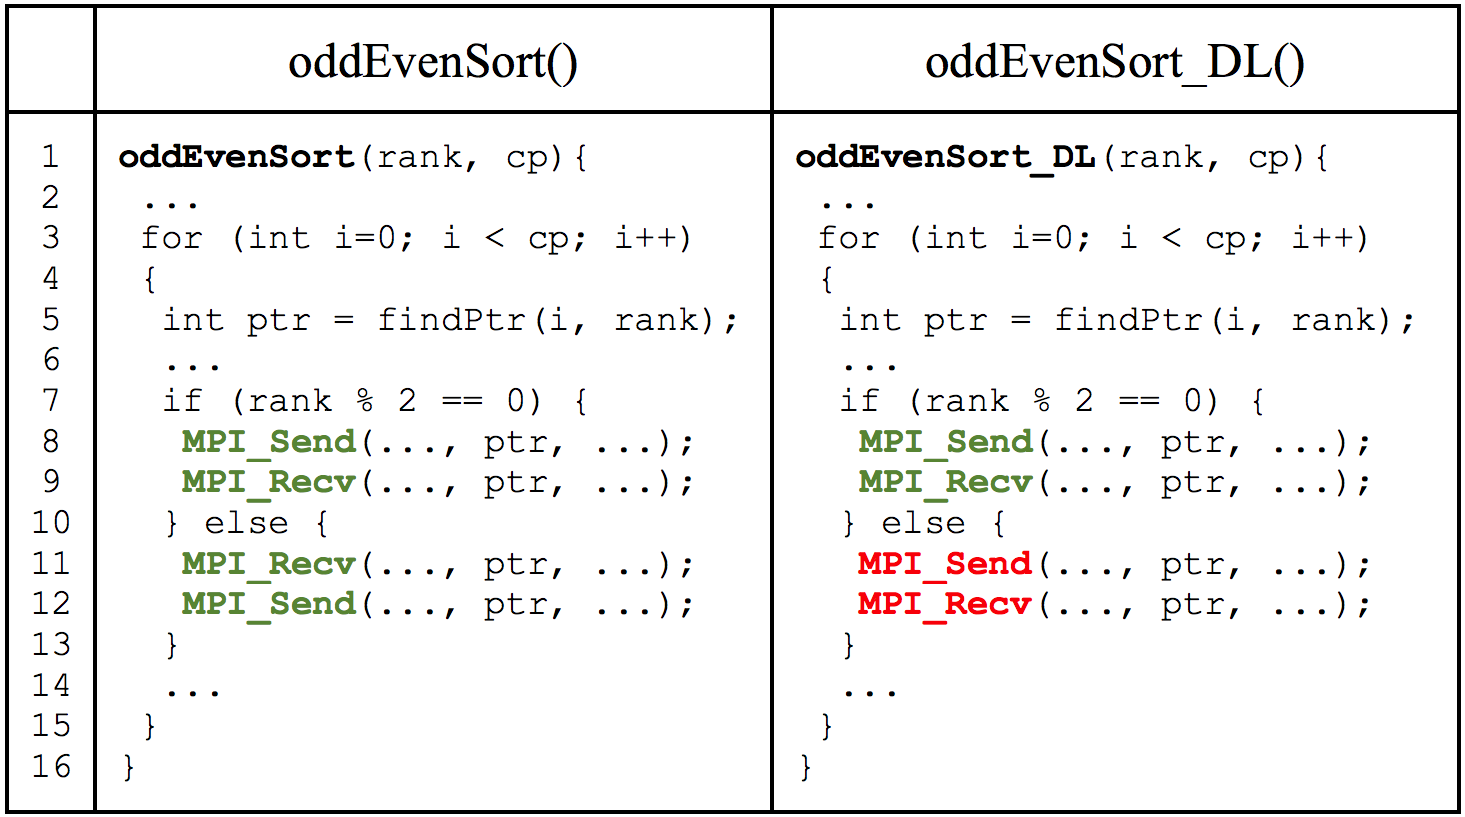
\includegraphics[width=0.45\textwidth]{figs/oddEvenDL.png}
%\label{fig.oddEvenDL}
%\end{figure}


\begin{frame}{}
  \lstset{language=C}
 \begin{lstlisting}[caption={ILCS Overview},label={lst:ilcs}]
main(argc, argv) {
 ... // initialization
 MPI_Init();
 MPI_Comm_size();
 MPI_Comm_rank(my_rank);
 ... // Obtain number of local CPUs and GPUs
 MPI_Reduce(lCPUs, gCPUs, MPI_SUM); // Total # of CPUs
 MPI_Reduce(lGPUs, gGPUs, MPI_SUM); // Total # of GPUs
 champSize = CPU_Init();
 ... // Memory allocation for storing local and global champions w.r.t. champSize
 MPI_Barrier();
 <@\textcolor{blue} {\#pragma omp parallel num\_threads(lCPUs+1)}@>
 {rank = omp_get_thread_num();
  if (rank != 0) { // worker threads
   while (cont) {
    ... // calculate seed
    local_result = CPU_Exec();
    if (local_result < champ[rank]) { // update local champion
     <@\textcolor{blue}{\#pragma omp critical}@>
     memcpy(champ[rank], local_result);}}
  } else { //master thread
   do {
    ...
    MPI_AllReduce(); //broadcast the global champion 
	  ...
    MPI_AllReduce(); //broadcast the global champion P_id
    ...
    if (my_rank == global_champion_P_id) {
     <@\textcolor{blue}{\#pragma omp critical}@>
     memcpy(bcast_buffer, champ[rank]);
    }
    MPI_Bcast(bcast_buffer); // broadcast the local champion to all nodes
   } while (no_change_threshold);
   cont = 0; // signal worker threads to terminate
  }}
 if (my_rank == 0) {CPU_Output(champ);}
 MPI_Finalize();}

/* User code for TSP problem */
CPU_Init() {/* Read coordinates, calculate distances, initialize champion structure, return structure size */}
CPU_Exec() {/* Find local champions (TSP tours) */}
CPU_Output() {/* Output champion */}
\end{lstlisting}
\end{frame}

\begin{table}[t]
\centering
\caption{Ranking table - OpenMP bug: unprotected shared memory access by thread 4 of process 6}
\label{tab:mc1-mc-6-4}
\scalebox{0.78}{
\begin{tabular}{|c|c|c|c|c|}
\hline
 Filter                           & Attributes   &   B-score & \begin{tabular}[c]{@{}c@{}}Top\\Processes\end{tabular}          & \begin{tabular}[c]{@{}c@{}}Top\\Threads\end{tabular}  \\
\hline
 11.plt.mem.cust.0K10             & doub.noFreq  &     0.244 & 7, 3, 4         & \textbf{6.4}, 7.3, 1.4, 3.3, 3.4, 4.2  \\
 11.plt.mem.cust.0K10             & doub.log10   &     0.244 & 7, 3, 4         & \textbf{6.4}, 7.3, 1.4, 3.3, 3.4, 4.2  \\
 01.plt.mem.cust.0K10             & doub.noFreq  &     0.244 & 7, 3, 4         & \textbf{6.4}, 7.3, 1.4, 3.3, 3.4, 4.2  \\
 01.plt.mem.cust.0K10             & doub.log10   &     0.244 & 7, 3, 4         & \textbf{6.4}, 7.3, 1.4, 3.3, 3.4, 4.2  \\
 01.mem.ompcrit.cust.0K10         & sing.log10   &     0.262 & 3                 & \textbf{6.4}, 7.1, 3.3, 4.1, 5.1, 6.1  \\
 01.mem.ompcrit.cust.0K10         & sing.noFreq  &     0.262 & 3                 & \textbf{6.4}, 7.1, 3.3, 4.1, 5.1, 6.1  \\
 11.mem.ompcrit.cust.0K10         & sing.log10   &     0.262 & 3                 & \textbf{6.4}, 7.1, 3.3, 4.1, 5.1, 6.1  \\
 11.mem.ompcrit.cust.0K10         & sing.noFreq  &     0.262 & 3                 & \textbf{6.4}, 7.1, 3.3, 4.1, 5.1, 6.1  \\
% 01.plt.mem.mpi.ompall.cust.0K10  & sing.actual  &     0.266 &                    & 2.4 , 4.3 ,                         \\
% 11.plt.mem.mpi.ompall.cust.0K10  & sing.actual  &     0.266 &                    & 2.4 , 4.3 ,                         \\
 11.plt.mem.cust.0K10             & doub.actual  &     0.273 & 7                 & \textbf{6.4}, 2.4, 3.4, 4.2, 4.4        \\
 01.plt.mem.cust.0K10             & doub.actual  &     0.273 & 7                 & \textbf{6.4}, 2.4, 3.4, 4.2, 4.4        \\
% 11.plt.mem.mpi.ompcrit.cust.0K10 & doub.noFreq  &     0.276 & 3 ,                & 3.3 , \textbf{6.4} ,                         \\
% 11.plt.mem.mpi.ompcrit.cust.0K10 & doub.log10   &     0.276 & 3 ,                & 3.3 , \textbf{6.4} ,                         \\
% 01.plt.mem.mpi.ompcrit.cust.0K10 & doub.noFreq  &     0.276 & 3 ,                & 3.3 , \textbf{6.4} ,                         \\
% 01.plt.mem.mpi.ompcrit.cust.0K10 & doub.log10   &     0.276 & 3 ,                & 3.3 , \textbf{6.4} ,                         \\
\hline
\end{tabular}}
\end{table}


\begin{table}[b]
\centering
\caption{Ranking table - MPI bug: wrong collective size in process 2}
\label{tab:ar1-ws-all-nn}
\scalebox{0.81}{
\begin{tabular}{|c|c|c|c|c|}
\hline
 Filter              & Attributes   &    B-score & \begin{tabular}[c]{@{}c@{}}Top\\Processes\end{tabular}          & \begin{tabular}[c]{@{}c@{}}Top\\Threads\end{tabular}         \\
\hline
% 11.mem.mpicol.ompcrit.cust.0K10 & sing.log10   &      0.383 & 0 , 7 , 2 , 4 , 5 , 6 , & 1.1 , 1.3 , 1.4 , 3.1 , 3.2 , 3.4 , \\
% 11.mem.mpicol.ompcrit.cust.0K10 & sing.noFreq  &      0.383 & 0 , 7 , 2 , 4 , 5 , 6 , & 1.1 , 1.3 , 1.4 , 3.1 , 3.2 , 3.4 , \\
 11.mpicol.cust.0K10             & sing.log10   &      0.439 & 0, 7, 2, 4, 5, 6  & 1.1, 1.3, 3.1, 3.2, 3.4        \\
 11.mpicol.cust.0K10             & sing.noFreq  &      0.439 & 0, 7, 2, 4, 5, 6  & 1.1, 1.3, 3.1, 3.2, 3.4        \\
 11.mpi.cust.0K10                & doub.noFreq  &      0.457 & 0, 7, 2, 4, 5, 6  & 1.4, 3.3, 3.4                    \\
 11.mpi.cust.0K10                & doub.actual  &      0.457 & 0, 7, 2, 4, 5, 6  & 1.4, 3.3, 3.4                    \\
 11.mpiall.cust.0K10             & doub.noFreq  &      0.457 & 0, 7, 2, 4, 5, 6  & 1.4, 3.3, 3.4                    \\
 11.mpiall.cust.0K10             & doub.actual  &      0.457 & 0, 7, 2, 4, 5, 6  & 1.4, 3.3, 3.4                    \\
 11.mpicol.cust.0K10             & doub.noFreq  &      0.457 & 0, 7, 2, 4, 5, 6  & 1.4, 3.3, 3.4                    \\
 11.mpicol.cust.0K10             & doub.actual  &      0.457 & 0, 7, 2, 4, 5, 6  & 1.4, 3.3, 3.4                    \\
 11.mpi.cust.0K10                & sing.log10   &      0.465 & 0, 7, 2, 4, 5, 6  & 1.1, 1.3, 3.1, 3.2, 3.4        \\
 11.mpi.cust.0K10                & sing.noFreq  &      0.465 & 0, 7, 2, 4, 5, 6  & 1.1, 1.3, 3.1, 3.2, 3.4        \\
 11.mpiall.cust.0K10             & sing.log10   &      0.465 & 0, 7, 2, 4, 5, 6  & 1.1, 1.3, 3.1, 3.2, 3.4        \\
 11.mpiall.cust.0K10             & sing.noFreq  &      0.465 & 0, 7, 2, 4, 5, 6  & 1.1, 1.3, 3.1, 3.2, 3.4        \\
 11.mpi.cust.0K10                & doub.noFreq  &      0.543 & 0, 7, 2, 4, 5, 6  & 1.4, 3.3, 3.4                    \\
 11.mpi.cust.0K10                & doub.actual  &      0.543 & 0, 7, 2, 4, 5, 6  & 1.4, 3.3, 3.4                    \\
\hline
\end{tabular}}
\end{table}

\begin{table}[b]
\centering
\caption{Ranking Table - MPI-Bug: Wrong Collective Operation ,Injected to Process 0}
\label{tab:ar1-wo-0-nn}
\scalebox{0.81}{
\begin{tabular}{|c|c|c|c|c|}
\hline
 Filter              & Attributes   &    B-score & \begin{tabular}[c]{@{}c@{}}Top\\Processes\end{tabular}          & \begin{tabular}[c]{@{}c@{}}Top\\Threads\end{tabular}  \\
\hline
 01.plt.cust.0K10    & doub.log10   &      0.271 & 2                 & 6.2, 7.3, 2.2, 5.2, 5.3  \\
 11.plt.cust.0K10    & doub.log10   &      0.271 & 2                 & 6.2, 7.3, 2.2, 5.2, 5.3  \\
 01.plt.cust.0K10    & sing.actual  &      0.276 & 1                 & 3.1, 1.4, 6.4, 3.4        \\
 11.plt.cust.0K10    & sing.actual  &      0.276 & 1                 & 3.1, 1.4, 6.4, 3.4        \\
 01.plt.cust.0K10    & doub.noFreq  &      0.285 & 2                 & 6.2, 7.3, 2.2, 5.2, 5.3  \\
 11.plt.cust.0K10    & doub.noFreq  &      0.285 & 2                 & 6.2, 7.3, 2.2, 5.2, 5.3  \\
 01.plt.cust.0K10    & sing.log10   &      0.292 & 1, 4, 5  & 3.1, 4.3                    \\
 11.plt.cust.0K10    & sing.log10   &      0.292 & 1, 4, 5   & 3.1, 4.3                    \\
 01.\textbf{mpicol}.cust.0K10 & sing.actual  &      0.312 & \textbf{5}                 & 3.2, 6.4, 5.4, 4.2        \\
 11.\textbf{mpicol}.cust.0K10 & sing.actual  &      0.312 & \textbf{5}                 & 3.2, 6.4, 5.4, 4.2        \\
 11.\textbf{mpi}.cust.0K10    & sing.actual  &      0.331 & \textbf{5}                 & 3.2, 6.4, 5.4, 4.2        \\
 11.\textbf{mpiall}.cust.0K10 & sing.actual  &      0.331 & \textbf{5}                 & 3.2, 6.4, 5.4, 4.2        \\
 01.\textbf{mpiall}.cust.0K10 & sing.actual  &      0.331 & \textbf{5}                 & 3.2, 6.4, 5.4, 4.2        \\
 01.\textbf{mpi}.cust.0K10    & sing.actual  &      0.331 & \textbf{5}                 & 3.2, 6.4, 5.4, 4.2        \\
 11.\textbf{mpi}.cust.0K10    & sing.actual  &      0.371 & \textbf{5}                 & 3.2, 6.4, 5.4, 4.2        \\
 11.\textbf{mpiall}.cust.0K10 & sing.actual  &      0.371 & \textbf{5}                 & 3.2, 6.4, 5.4, 4.2        \\
\hline
\end{tabular}}
\end{table}



\section{Algorithms Underlying DiffTrace}
\label{sec:ch3_algo}
\subsection{Nested Loop Recognition (NLR)}
\label{subsec:algo-nlr}

We build NLRs based on the work by Ketterlin and Clauss~\cite{Ketterlin-nlr},
who use this algorithm for trace compression,
and the work by Kobayashi and MacDougall~\cite{kobayashi-84}, who propose
a similar bottom-up strategy to build loop nests from traces,
replacing each recognized loop with a new symbol.
%(sequence of string instructions) where each
%is originally designed for prediction and compression of data access traces (memory addresses) through detecting the ``linear progression function'' in the sequence of addresses.
%
%Two main operations of NLR algorithm are 1) recognizing the start of a loop and forming its initial syntactic structure and 2) recognizing if what follows a loop is just another iteration and extend the upper bound.
%
%These operations are performed incrementally and recursively to recognize loops at different depths (i.e., a linear function of the loop index and depth) until the input sequence is completely consumed and no more loop is detected.
%
%
%we have re-implemented the NLR algorithm (DiffTrace-NLR) for detecting repetitive patterns
We adapt these algorithms
to function-call traces
wherein we record
identical loops at different locations by introducing
a single new (made-up) function ID that represents the entire loop.
%
This process is restarted once the whole trace has been analyzed for depth-2 loops and so on until a function-ID replacement is performed.
%
DiffTrace-NLR works by incrementally pushing trace entries (function IDs)
onto a stack of \textit{elements} (i.e., function IDs
representing detected loop structures).
%
Whenever an element is pushed onto the stack $S$,
the upper elements of the stack are recursively
examined for potential loop detection or loop extensions (Procedure \ref{proc:NLR}).


\begin{small}
\begin{algorithm}[]
 \DontPrintSemicolon
 \SetKwFunction{KwReduce}{Reduce}
% \SetKwInOut{Input}{Input} \SetKwInOut{Output}{Output}\SetKwInOut{Local}{Local}
  %\SetKw{KwEach}{each}
 %\Input{Stack of elements $S$, $S[1]$ is top}
 %\Output{$NLR(T)$}
 \KwReduce{$S$}:{\\
 \Indp
     \For{$ i:1$ ... $3K$}{
         $b$ = $i/3$\;
         \If{Top 3 $b$-long elements of $S$ are \textit{isomorphic}}{
             pop $i$ elements from $S$\;
             $LB=S[b:1]$,
             $LC=3$\;
             $LS=(LB,LC)$\;
             push $LS$ to $S$\;
             add $LB$ to the Loop Table\;
             \KwReduce{$S$}\;
         }
         \If{ $S[i]$ is a loop ($LS$) and $S[i-1:1]$ isomorphic to its loop body$LB$}{
             $LC=LC+1$\;
             pop $i-1$ elements from $S$\;
             \KwReduce{$S$}\;
         }
     }
 }

 \caption{\texttt{Reduce} procedure adapted from the NLR algorithm }
 \label{proc:NLR}
\end{algorithm}
\end{small}

% Each loop structure \textbf{LS} is a tuple of (loop body \textbf{LB}, loop count \textbf{LC}) where LB is a sequence of elements, and LC is an integer showing the frequency of consecutive occurrence of LB.
% %
% To avoid coincidental regularity, the algorithm needs at least \textit{three} consecutive terms to form an LS.
% %
% The \texttt{Reduce} procedure checks to see if any three consecutive subsequences on top of the stack are \textit{isomorphic}.
% %
% In our context, two sequences are isomorphic if both have equal lengths and identical corresponding elements.
% %
% If the check passes, then the top three consecutive subsequences (LB) are popped from the stack, and the LS=(LB,3) is pushed onto the stack. Otherwise, top elements of the stack are compared against the potential LS behind them to increment the LC in case of isomorphism.
% If either of the above examinations succeeds, the procedure restarts on the recently modified stack for detecting or extending potential nested loops.
%

We store all distinct loop bodies (LBs)
in a hash-table, assigning each a unique ID, which can be applied as
a heuristic to detect loops not only in the current trace but also in other
traces of the same execution.
%
The maximum length of the subsequences to examine is decided by a fixed $K$.
%
The complexity of the NLR algorithm is $\Theta(K^2N)$ where $N$ is the size of the input.
%
While loop detection has been researched in other contexts,
its use to support debugging is believed to be novel.

\subsection{Concept Lattice Construction}
\label{subsec:algo-cl}

%There exist algorithms that extract concepts and their partial order from a formal context; each has its pros and cons.
%
The efficiency of algorithms for concept lattice construction
depends on the sparseness of the formal context~\cite{clgenperform}.
%
%Based on the sparseness of the formal context,
%the
%
Ganter's \textit{Next Closure} algorithm \cite{clbook}
constructs the lattice from a
\textit{batch} of contexts and requires the whole context to be present in main memory and is, therefore, inefficient for long HPC traces.
%
%For large scale HPC traces, such an approach is inefficient.
%


% Please add the following required packages to your document preamble:
% \usepackage{multirow}
\begin{table}[]
\caption{Attributes mined from traces}
\label{tab:atr}
\centering
\scalebox{0.9}{
\begin{tabular}{|l|l|c|l|}
\hline
\multicolumn{4}{|c|}{\begin{tabular}[c]{@{}c@{}}\textbf{Attributes}\\ \{attr:freq\}\end{tabular}} \\ \hline
\multicolumn{2}{|c|}{attr} & \multicolumn{2}{c|}{freq} \\ \hline
\multirow{3}{*}{\textbf{Single}} & \multirow{3}{*}{\begin{tabular}[c]{@{}l@{}}each entry \\ of the trace\end{tabular}} & \multirow{2}{*}{\textbf{Actual}} & \multirow{2}{*}{observed frequency} \\
 &  &  &  \\ \cline{3-4} 
 &  & \multirow{2}{*}{\textbf{Log10}} & \multirow{2}{*}{log10 of the observed frequency} \\ \cline{1-2}
\multirow{3}{*}{\textbf{Double}} & \multirow{3}{*}{\begin{tabular}[c]{@{}l@{}}each pair of \\ consecutive entries\end{tabular}} &  &  \\ \cline{3-4} 
 &  & \multirow{2}{*}{\textbf{noFreq}} & \multirow{2}{*}{no frequency} \\
 &  &  &  \\ \hline
\end{tabular}}
\end{table}

%
We have implemented Godin's \textit{incremental} algorithm \cite{clconst}
to extract attributes (Table \ref{tab:atr})
from each trace (object) and inject them into an initially empty lattice.
%
Notice that our representation already includes compression of the attributes as (1) either the
observed frequency is recorded, (2) the log10 of the frequency is recorded, or (3) ``no frequency''
(presence/absence) of a function call is recorded.
%
{\em These are versatile knobs to adjust for bug-location and similarity calculation}.


Every time a new object with its set of attributes is added to the lattice,
an \textit{update} procedure minimally modifies/adds/deletes edges and nodes of the lattice.
%
%This procedure is guaranteed to preserve the validity of the concept lattice properties.
%
The extracted attributes are in the form \textit{\{attr:freq\}}.
%
\textit{attr} is either a single entry of the trace NLR or a consecutive pair of entries.
\textit{freq} is a parameter to adjust the impact of the frequency of each \textit{attr}
in the concept lattice.
%
The complexity of Godin's algorithm is $O(2^{2K}|G|)$, where $K$ is an upper bound for the number of attributes (e.g., distinct function calls in the whole execution) and $|G|$ is the number of objects (e.g., the number of traces).

%In DiffTrace, the upper bound for the number of attributes is usually small since traces are pre-processed and summarized in the form of NLRs. Thus Godin's algorithm would perform near



\subsection{Hierarchical Clustering, Construction, and Comparison}
\label{subsec:algo-bscore}

 DiffJSMs provide pair-wise dissimilarity
 measurements that can be used to combine traces (forming initial clusters).
%
% However, to derive a flat clustering of traces to detect the outlier(s)
To obtain outliers (suspicious traces),
we form dendrograms for which
a \textit{linkage} function is required to measure the distance between sets of traces.
%
 We currently employ SciPy (version 1.3.0. \cite{scipy}) for these tasks.
% for clustering and obtaining
% the table of suspicious traces.
%derived from the DiffJSM by hierarchical clustering algorithms in
%
%
 SciPy provides a wide range of linkage functions
 such as single, complete, average, weighted, centroid, median, and ward.

\subsubsection{Ranking Table}
As shown in Figure \ref{fig.diffTraceOverview},
each component of DiffTrace has some tunable parameters and constants,
and the suggested suspicious traces are a function of them.
%
Thus, a metric is needed to serve as the sorting key of the suspicious traces.
%
Each parameter combination, in essence, creates a different DiffJSM,
giving us ``the distance between two hierarchical clusterings''.
%
Fowlkes et al.~\cite{fowlkes83} proposed a method for comparing two
hierarchical clusterings by computing their \textit{B-score}.
%
%The B-score of two clusterings is computed by counting the number of objects that fall into different clusters.
%%
While we have not evaluated the full relevance of this idea,
our initial experiments show that sorting suspicious traces based on the B-score of DiffJSMs is
effective and brings interesting outliers to attention.
%--end


\section{Case Study: ILCS}
\label{sec:ch3_ilcs-case-study}




ILCS is a scalable framework for running iterative local searches on HPC platforms~\cite{ilcs}.
%
Providing serial CPU and/or single-GPU code, ILCS executes this code in parallel between compute nodes (MPI) and within them (OpenMP and CUDA).
%

To evaluate DiffTrace, we manually injected MPI-level and OMP-level bugs into the Traveling Salesman Problem (TSP) running on ILCS (Listing~\ref{lst:ilcs}).
%
The injected bugs simulate real HPC bugs such as deadlocks.
%
%These bugs are close to common mistakes that HPC developers usually make during developing HPC codes.
%
Moreover, we inserted ``hidden'' faults that do not crash the program such as violations of critical sections and semantic bugs.
%
%The injected bugs are planted in a way that might get triggered in only one or more threads (master and worker threads, one thread, every other thread, all threads except one, all threads).
%
The goal was to see how effectively DiffTrace can analyze the resulting traces and how close it can get to the root cause of the fault.
%


%
We collected ParLOT (main image) traces from the execution of ILCS-TSP with 8 MPI processes and 4 OpenMP threads per process on the XSEDE-PSC Bridges supercomputer whose compute nodes have 128 GB of main memory and contain 2 Intel Haswell (E5-2695 v3) CPUs with 14 cores each running at 2.3 - 3.3 GHz.
%
Note that we did not provide any GPU code to ILCS.
%

The collected traces (faulty and normal) are fed to DiffTrace. We enabled the MPI, OpenMP, and custom (ILCS-TSP user code) filters and set the NLR constant K to 10 for all experiments.
%
The current version of DiffTrace is implemented and built using C++ GCC 5.5.0, Pin 3.8, Python 2.7, and Scipy 1.3.0.

%
We present the results in the form of ranking tables that show which traces (processes and threads) DiffTrace considers ``suspicious''. Since DiffTrace output is highly dependent to ``parameters'', each row in ranking tables starts with parameters whom the suspicious traces are the result of.

The linkage method that converts JSMs to flat clustering is ``ward'' for all of the top reported suspicious traces that we removed from tables for better readability. Ward linkage function in SciPy uses \textit{Ward variance minimization algorithm} to calculate the distance between newly formed clusters~\cite{scipy}. Furthermore, we show diffNLRs for selected traces.



\subsection{ILCS-TSP Workflow}

The TSP code starts with a random tour and iteratively shortens it using the 2-opt improvement heuristic~\cite{2-opt} until a local minimum is reached. ILCS automatically and asynchronously distributes unique seed values to each worker thread, runs the TSP code, reduces the results to find the best solution, and repeats these steps until the termination criterion is met. It employs two types of threads per node: a \textit{master} thread (MPI process) that handles the communication and local work distribution and a set of \textit{worker} threads (OpenMP threads) that execute the provided TSP code. The master thread forks a worker thread for each detected CPU core.
%
Each worker thread continually calls
\texttt{CPU\_Exec()} to evaluate a seed and records the result (lines 14-20).
%
Once the worker threads are running, the master thread's primary job is to scan the results of the workers to find the best solution computed so far (i.e., the local champion). This information is then globally reduced to determine the current system-wide champion (lines 22-32).
%
ILCS terminates the search when the quality has not improved over a certain period (lines 33-34).



\subsection{OpenMP Bug: Unprotected Memory Access}

The memory accesses performed by the \texttt{memcpy} calls on lines 20 and 30 are protected by an OpenMP critical section.
%
Not protecting them results in a data race that might lead to incorrect final program output.
%
To simulate this scenario, we modified the ILCS source code to omit the critical section in worker thread 4 of process 6.

Table~\ref{tab:mc1-mc-6-4} lists the top suspicious traces that DiffTrace finds when injecting this bug.
%
Each row presents the results for different filters and attributes.
%
For example, the filter ``11.mem.ompcit.cust.0K10'' removes all function returns and .plt calls from the traces and only keeps memory-related calls, OpenMP critical-section functions, and the custom function ``CPU\_Exec''.
%
The ``K10'' at the end of filter means that the filtered traces are converted into an NLR with $K$=10.
%
%\hl{I will remove two unnecessary columns from the tables (threshold and linkage function) to save space and add 2-3 sentences explaining what was them}
%
The bold numbers in the rightmost column of the table flag trace 6.4 (i.e., process 6, thread 4) as the trace that was affected the most by the bug.
%

The corresponding diffNLR(6.4) presented in Figure~\ref{diffNLR-6-4} clearly shows that the normal execution of ILCS (green and blue blocks) protects the \texttt{memcpy} while the buggy execution (green and red blocks) does not. Here, L0 represents \texttt{CPU\_Exec}, which is called multiple times in both the fault-free and the buggy version (the call frequencies are different due to the asynchronous nature of ILCS).
%


%\begin{figure}[]
%\centering
%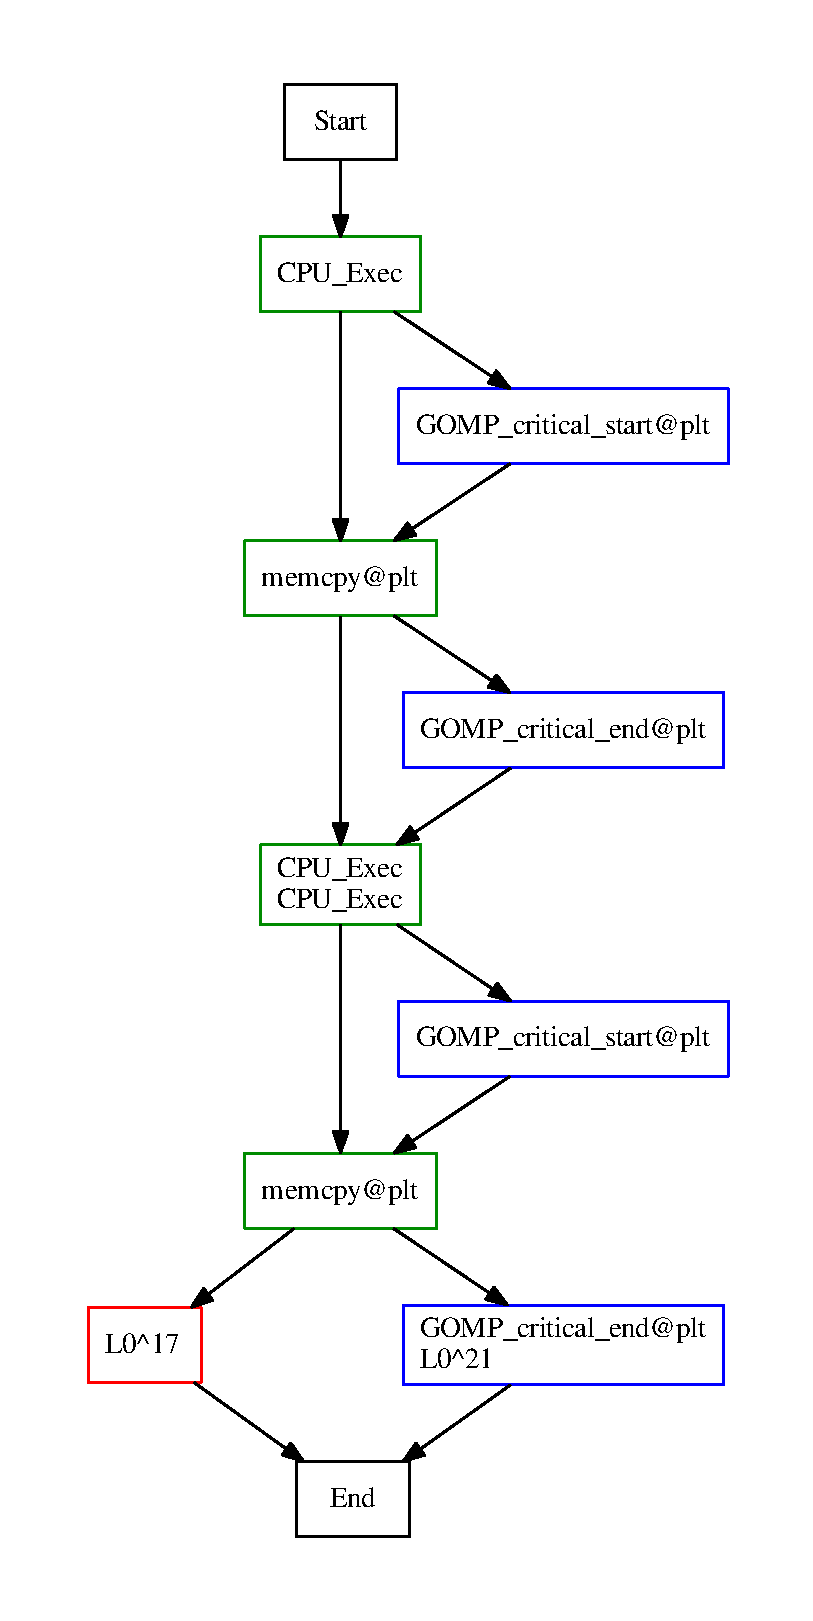
\includegraphics[width=0.3\textwidth]{figs/diffNLR/ompBug-6-4.pdf}
%\caption{OpenMP Bug: diffNLR(6.4)}
%\label{diffNLR-6-4}
%\end{figure}


\subsection{MPI Bug: Deadlock Caused by Fault in Collective}

By forcing process 2 to invoke MPI\_Allreduce (line 24) with a wrong size, we can inject a \textit{real deadlock}.
%
Because the deadlock happens early in the execution, the resulting traces are very different from their fault-free counterparts.
%
Consequently, DiffTrace marks almost all processes as suspicious (cf.~Table~\ref{tab:ar1-ws-all-nn}).
%
Clearly, this is not helpful for debugging.
%
Nevertheless, diffNLR still yields useful information.
%
Since most of the traces are suspicious, we do not know which one the real culprit is and randomly selected trace~4.
%
%It turned out that ParLoT did not happen to capture function calls from all processes since the bug happens too early in the code. Thus except for process 1 and 4, all other traces are empty.
%
By looking at the diffNLR(4) output shown in Figure~\ref{diffNLR-0}, we immediately see that both the normal and the buggy trace are identical up to the invocation of MPI\_Allreduce. This gives the user the first (correct) hint as to where the problem lies.
%
Beyond this point, the bug-free process continues to the end of the program
(it reaches the MPI\_Finalize call) whereas the buggy process does not. The last entry in the buggy trace is a call to MPI\_Allreduce (the last green box), indicating that this call never returned, that is, it deadlocked. This provides the user with the second (correct) hint as to the type of the underlying bug.
%

%
\begin{table}[b]
\centering
\caption{Ranking table - MPI bug: wrong collective size in process 2}
\label{tab:ar1-ws-all-nn}
\scalebox{0.81}{
\begin{tabular}{|c|c|c|c|c|}
\hline
 Filter              & Attributes   &    B-score & \begin{tabular}[c]{@{}c@{}}Top\\Processes\end{tabular}          & \begin{tabular}[c]{@{}c@{}}Top\\Threads\end{tabular}         \\
\hline
% 11.mem.mpicol.ompcrit.cust.0K10 & sing.log10   &      0.383 & 0 , 7 , 2 , 4 , 5 , 6 , & 1.1 , 1.3 , 1.4 , 3.1 , 3.2 , 3.4 , \\
% 11.mem.mpicol.ompcrit.cust.0K10 & sing.noFreq  &      0.383 & 0 , 7 , 2 , 4 , 5 , 6 , & 1.1 , 1.3 , 1.4 , 3.1 , 3.2 , 3.4 , \\
 11.mpicol.cust.0K10             & sing.log10   &      0.439 & 0, 7, 2, 4, 5, 6  & 1.1, 1.3, 3.1, 3.2, 3.4        \\
 11.mpicol.cust.0K10             & sing.noFreq  &      0.439 & 0, 7, 2, 4, 5, 6  & 1.1, 1.3, 3.1, 3.2, 3.4        \\
 11.mpi.cust.0K10                & doub.noFreq  &      0.457 & 0, 7, 2, 4, 5, 6  & 1.4, 3.3, 3.4                    \\
 11.mpi.cust.0K10                & doub.actual  &      0.457 & 0, 7, 2, 4, 5, 6  & 1.4, 3.3, 3.4                    \\
 11.mpiall.cust.0K10             & doub.noFreq  &      0.457 & 0, 7, 2, 4, 5, 6  & 1.4, 3.3, 3.4                    \\
 11.mpiall.cust.0K10             & doub.actual  &      0.457 & 0, 7, 2, 4, 5, 6  & 1.4, 3.3, 3.4                    \\
 11.mpicol.cust.0K10             & doub.noFreq  &      0.457 & 0, 7, 2, 4, 5, 6  & 1.4, 3.3, 3.4                    \\
 11.mpicol.cust.0K10             & doub.actual  &      0.457 & 0, 7, 2, 4, 5, 6  & 1.4, 3.3, 3.4                    \\
 11.mpi.cust.0K10                & sing.log10   &      0.465 & 0, 7, 2, 4, 5, 6  & 1.1, 1.3, 3.1, 3.2, 3.4        \\
 11.mpi.cust.0K10                & sing.noFreq  &      0.465 & 0, 7, 2, 4, 5, 6  & 1.1, 1.3, 3.1, 3.2, 3.4        \\
 11.mpiall.cust.0K10             & sing.log10   &      0.465 & 0, 7, 2, 4, 5, 6  & 1.1, 1.3, 3.1, 3.2, 3.4        \\
 11.mpiall.cust.0K10             & sing.noFreq  &      0.465 & 0, 7, 2, 4, 5, 6  & 1.1, 1.3, 3.1, 3.2, 3.4        \\
 11.mpi.cust.0K10                & doub.noFreq  &      0.543 & 0, 7, 2, 4, 5, 6  & 1.4, 3.3, 3.4                    \\
 11.mpi.cust.0K10                & doub.actual  &      0.543 & 0, 7, 2, 4, 5, 6  & 1.4, 3.3, 3.4                    \\
\hline
\end{tabular}}
\end{table}


%\begin{figure}[]
%\centering
%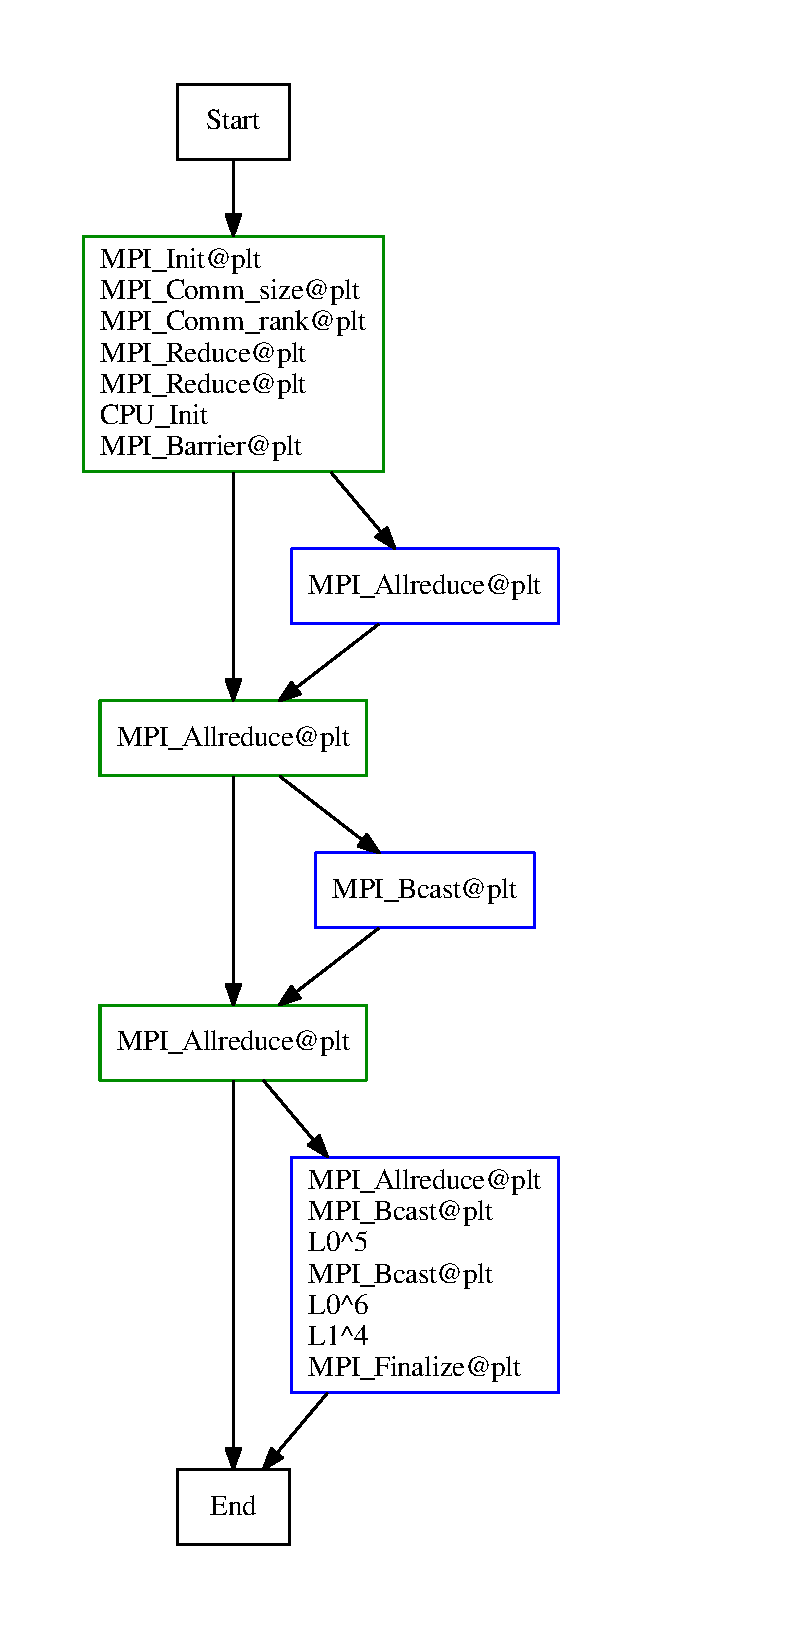
\includegraphics[width=0.3\textwidth]{figs/diffNLR/mpiBug-all-nn.pdf}
%\caption{diffNLR(0)}
%\label{diffNLR-0}
%\end{figure}
%





\subsection{MPI Bug: Wrong Collective Operation}

By changing the MPI\_MIN argument to MPI\_MAX in the MPI\_Allreduce call on line 24 of Listing~\ref{lst:ilcs}, the semantics of ILCS change.
%
Instead of computing the best answer, the modified code computes the worst answer.
%
Hence, this code variation terminates but is likely to yield the wrong result.
%
We injected this bug into process 0.

The first few suspicious processes listed in Table~\ref{tab:ar1-wo-0-nn} are inconclusive. However, the filters that include MPI all agree that process 5 changed the most.
%
Looking at the corresponding diffNLR(5) output in Figure~\ref{diffNLR-5} makes it clear why process 5 was singled out. In the buggy run, it executes many more MPI\_Bcast calls than in the bug-free run because the frequency in which local ``optimums'' are produced has changed. Though this should affect all traces equally, which has reflected in the diffNLR of other traces. We are presenting these tables and figures to show that DiffTrace can reveal the impact of silent bugs like the wrong operation. Such data representation via suggested tables and diffNLRs helps developers to gain insight into the general behavior of the execution. More accurate results can be obtained by refining the parameters and collecting more profound traces (e.g., ParLOT(all images)). This would be part of our future work to find the set of parameters for different classes of bugs to maximize accuracy.



%\begin{figure}[]
%\centering
%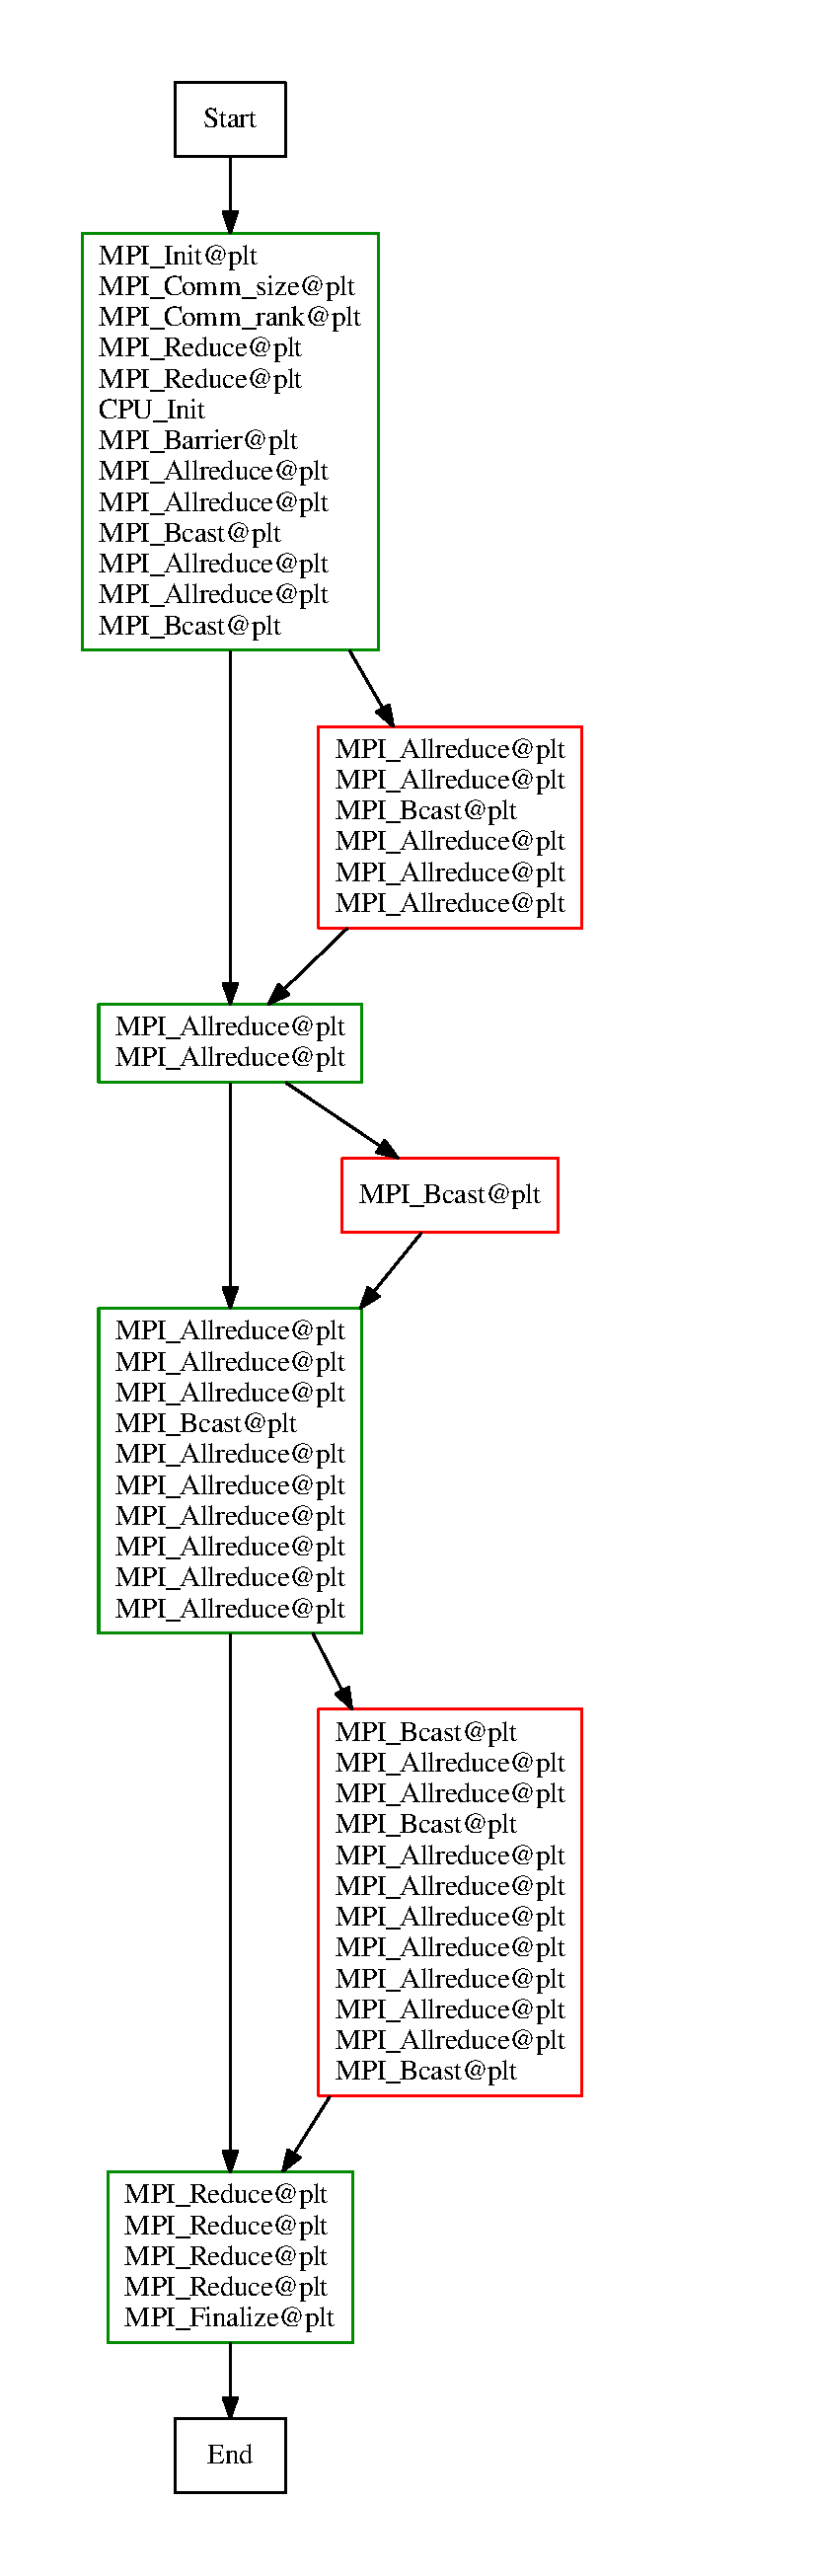
\includegraphics[width=0.3\textwidth]{figs/diffNLR/mpiBug2-0-nn.pdf}
%\caption{diffNLR(5)}
%\label{diffNLR-5}
%\end{figure}

%\begin{table}[]
\centering
\caption{ilcsTSP.mc1-mc-6-n1.m.8.auto}
\label{s1}
\scalebox{0.5}{
\begin{tabular}{lllrrll}
\hline
 Filter                           & Attributes   & Link Method   &   Thresh &   B-score & Top Procs (JSMD)   & TOP Threads(JSMD)                   \\
\hline
 01.mem.ompall.cust.0K10          & sing.actual  & average       &        4 &  0.308594 &                    & 6.2 , 6.4 , 5.2 , 5.4 , 7.3 ,       \\
 11.mem.ompall.cust.0K10          & sing.actual  & average       &        4 &  0.308594 &                    & 6.2 , 6.4 , 5.2 , 5.4 , 7.3 ,       \\
 01.mem.ompmutex.cust.0K10        & sing.actual  & weighted      &        4 &  0.321883 &                    & 6.2 , 3.4 , 5.3 , 4.2 , 7.4 ,       \\
 11.mem.ompmutex.cust.0K10        & sing.actual  & weighted      &        4 &  0.321883 &                    & 6.2 , 3.4 , 5.3 , 4.2 , 7.4 ,       \\
 11.plt.mem.mpi.ompcrit.cust.0K10 & doub.actual  & weighted      &        4 &  0.324427 & 3 ,                & 0.2 , 1.1 , 3.1 , 4.3 , 4.4 , 5.2 , \\
 01.plt.mem.mpi.ompcrit.cust.0K10 & doub.actual  & weighted      &        4 &  0.324427 & 3 ,                & 0.2 , 1.1 , 3.1 , 4.3 , 4.4 , 5.2 , \\
 01.mem.ompall.cust.0K10          & doub.actual  & weighted      &        4 &  0.33266  & 3 ,                & 6.4 , 7.1 , 3.4 , 4.3 , 4.4 , 5.2 , \\
 11.mem.ompall.cust.0K10          & doub.actual  & weighted      &        4 &  0.33266  & 3 ,                & 6.4 , 7.1 , 3.4 , 4.3 , 4.4 , 5.2 , \\
 01.mem.ompcrit.cust.0K10         & sing.actual  & weighted      &        4 &  0.354396 & 6 ,                & 7.2 , 7.4 , 3.4 , 4.2 , 4.3 , 4.4 , \\
 11.mem.ompcrit.cust.0K10         & sing.actual  & weighted      &        4 &  0.354396 & 6 ,                & 7.2 , 7.4 , 3.4 , 4.2 , 4.3 , 4.4 , \\
 11.plt.mem.mpi.ompcrit.cust.0K10 & doub.actual  & average       &        4 &  0.381646 &                    & 3.3 , 2.4 ,                         \\
\hline
\end{tabular}}
\end{table}


\begin{table}[]
\centering
\caption{ilcsTSP.mc1-mc-2-2.m.8.auto}
\label{s2}
\scalebox{0.5}{
\begin{tabular}{lllrrll}
\hline
 Filter                           & Attributes   & Link Method   &   Thresh &   B-score & Top Procs (JSMD)   & TOP Threads(JSMD)                   \\
\hline
 01.mem.ompall.cust.0K10          & doub.actual  & weighted      &        4 &  0.309391 & 3 ,                & 6.2 , 6.4 , 7.1 , 7.4 , 1.3 , 3.1 , \\
 11.mem.ompall.cust.0K10          & doub.actual  & weighted      &        4 &  0.309391 & 3 ,                & 6.2 , 6.4 , 7.1 , 7.4 , 1.3 , 3.1 , \\
 11.plt.mem.cust.0K10             & doub.actual  & weighted      &        4 &  0.318003 & 7 , 4 ,            & 1.3 , 2.2 , 3.3 , 3.4 , 4.2 , 4.3 , \\
 01.plt.mem.cust.0K10             & doub.actual  & weighted      &        4 &  0.318003 & 7 , 4 ,            & 1.3 , 2.2 , 3.3 , 3.4 , 4.2 , 4.3 , \\
 01.mem.ompall.cust.0K10          & doub.actual  & average       &        4 &  0.34462  & 7 , 3 ,            & 7.1 , 1.3 , 1.4 , 2.2 , 2.3 , 3.1 , \\
 11.mem.ompall.cust.0K10          & doub.actual  & average       &        4 &  0.34462  & 7 , 3 ,            & 7.1 , 1.3 , 1.4 , 2.2 , 2.3 , 3.1 , \\
 11.plt.mem.mpi.ompcrit.cust.0K10 & doub.actual  & average       &        4 &  0.350702 & 7 , 3 ,            & 6.2 , 6.3 , 7.2 , 2.4 , 3.3 , 4.2 , \\
 01.plt.mem.mpi.ompcrit.cust.0K10 & doub.actual  & average       &        4 &  0.350702 & 7 , 3 ,            & 6.2 , 6.3 , 7.2 , 2.4 , 3.3 , 4.2 , \\
 11.plt.mem.cust.0K10             & doub.actual  & weighted      &        3 &  0.357334 & 7 ,                & 2.2 , 3.3 , 3.4 , 4.3 , 4.4 ,       \\
 01.plt.mem.cust.0K10             & doub.actual  & weighted      &        3 &  0.357334 & 7 ,                & 2.2 , 3.3 , 3.4 , 4.3 , 4.4 ,       \\
 01.mem.ompall.cust.0K10          & doub.actual  & weighted      &        3 &  0.380481 & 3 ,                & 7.1 , 1.3 , 3.1 , 4.3 , 4.4 ,       \\
\hline
\end{tabular}}
\end{table}


\begin{table}[]
\centering
\caption{ilcsTSP.ar2-wo-2-nn.m.8.auto}
\label{s3}
\scalebox{0.5}{
\begin{tabular}{lllrrll}
\hline
 Filter           & Attributes   & Link Method   &   Thresh &   B-score & Top Procs (JSMD)   & TOP Threads(JSMD)                   \\
\hline
 01.plt.cust.0K10 & doub.actual  & average       &        4 &  0.392446 & 6 ,                & 2.3 , 2.4 , 4.2 , 4.3 , 4.4 ,       \\
 11.plt.cust.0K10 & doub.actual  & average       &        4 &  0.392446 & 6 ,                & 2.3 , 2.4 , 4.2 , 4.3 , 4.4 ,       \\
 01.plt.cust.0K10 & sing.log10   & centroid      &        4 &  0.945946 & 0 ,                & 6.2 , 0.4 , 1.1 , 0.1 , 2.3 , 2.4 , \\
 01.plt.cust.0K10 & sing.log10   & median        &        4 &  0.945946 & 0 ,                & 6.2 , 0.4 , 1.1 , 0.1 , 2.3 , 2.4 , \\
 11.plt.cust.0K10 & sing.log10   & centroid      &        4 &  0.945946 & 0 ,                & 6.2 , 0.4 , 1.1 , 0.1 , 2.3 , 2.4 , \\
 11.plt.cust.0K10 & sing.log10   & median        &        4 &  0.945946 & 0 ,                & 6.2 , 0.4 , 1.1 , 0.1 , 2.3 , 2.4 , \\
 01.plt.cust.0K10 & sing.log10   & median        &        3 &  0.947368 & 0 ,                & 6.2 , 0.4 , 1.1 , 0.1 , 2.3 , 2.4 , \\
 11.plt.cust.0K10 & sing.log10   & median        &        3 &  0.947368 & 0 ,                & 6.2 , 0.4 , 1.1 , 0.1 , 2.3 , 2.4 , \\
 01.plt.cust.0K10 & sing.log10   & complete      &        3 &  1        & 0 ,                & 0.1 , 7.1 , 1.1 , 3.1 , 3.3 ,       \\
 01.plt.cust.0K10 & sing.log10   & complete      &        4 &  1        & 0 ,                & 0.1 , 7.1 , 1.1 , 3.1 , 3.3 ,       \\
 01.plt.cust.0K10 & sing.log10   & average       &        4 &  1        & 0 ,                & 0.1 , 7.1 , 1.1 , 3.1 , 3.3 ,       \\
\hline
\end{tabular}}
\end{table}


\begin{table}[]
\centering
\caption{ilcsTSP.bc2-wr-3-nn.m.8.auto}
\label{s4}
\scalebox{0.5}{
\begin{tabular}{lllrrll}
\hline
 Filter              & Attributes   & Link Method   &   Thresh &   B-score & Top Procs (JSMD)   & TOP Threads(JSMD)                   \\
\hline
 01.plt.cust.0K10    & doub.actual  & centroid      &        4 &  0.512309 & 2 ,                & 6.4 , 7.3 , 1.2 , 1.3 , 2.1 , 2.2 , \\
 11.plt.cust.0K10    & doub.actual  & centroid      &        4 &  0.512309 & 2 ,                & 6.4 , 7.3 , 1.2 , 1.3 , 2.1 , 2.2 , \\
 01.plt.cust.0K10    & sing.actual  & average       &        4 &  0.513221 & 7 ,                & 3.4 , 5.2 , 4.2 , 4.3 ,             \\
 11.plt.cust.0K10    & sing.actual  & average       &        4 &  0.513221 & 7 ,                & 3.4 , 5.2 , 4.2 , 4.3 ,             \\
 11.mpi.cust.0K10    & sing.actual  & median        &        4 &  0.544807 & 0 ,                & 0.1 , 6.4 , 7.3 , 7.4 , 1.3 , 0.2 , \\
 11.mpiall.cust.0K10 & sing.actual  & median        &        4 &  0.544807 & 0 ,                & 0.1 , 6.4 , 7.3 , 7.4 , 1.3 , 0.2 , \\
 01.mpiall.cust.0K10 & sing.actual  & median        &        4 &  0.544807 & 0 ,                & 0.1 , 6.4 , 7.3 , 7.4 , 1.3 , 0.2 , \\
 01.mpicol.cust.0K10 & sing.actual  & median        &        4 &  0.544807 & 0 ,                & 0.1 , 6.4 , 7.3 , 7.4 , 1.3 , 0.2 , \\
 11.mpicol.cust.0K10 & sing.actual  & median        &        4 &  0.544807 & 0 ,                & 0.1 , 6.4 , 7.3 , 7.4 , 1.3 , 0.2 , \\
 01.mpi.cust.0K10    & sing.actual  & median        &        4 &  0.544807 & 0 ,                & 0.1 , 6.4 , 7.3 , 7.4 , 1.3 , 0.2 , \\
 01.plt.cust.0K10    & doub.actual  & centroid      &        3 &  0.639268 & 2 ,                & 6.4 , 7.3 , 1.2 , 1.3 , 2.1 , 2.2 , \\
\hline
\end{tabular}}
\end{table}

\begin{table}[]
\centering
\caption{ilcsTSP.bc1-ws-3-nn.m.8.auto}
\label{s5}
\scalebox{0.5}{
\begin{tabular}{lllrrll}
\hline
 Filter              & Attributes   & Link Method   &   Thresh &   B-score & Top Procs (JSMD)   & TOP Threads(JSMD)                   \\
\hline
 11.mpi.cust.0K10    & sing.actual  & weighted      &        4 &  0.385229 & 6 ,                & 6.2 , 6.3 , 6.4 , 7.2 , 7.3 , 7.4 , \\
 11.mpiall.cust.0K10 & sing.actual  & weighted      &        4 &  0.385229 & 6 ,                & 6.2 , 6.3 , 6.4 , 7.2 , 7.3 , 7.4 , \\
 01.mpiall.cust.0K10 & sing.actual  & weighted      &        4 &  0.385229 & 6 ,                & 6.2 , 6.3 , 6.4 , 7.2 , 7.3 , 7.4 , \\
 01.mpicol.cust.0K10 & sing.actual  & weighted      &        4 &  0.385229 & 6 ,                & 6.2 , 6.3 , 6.4 , 7.2 , 7.3 , 7.4 , \\
 11.mpicol.cust.0K10 & sing.actual  & weighted      &        4 &  0.385229 & 6 ,                & 6.2 , 6.3 , 6.4 , 7.2 , 7.3 , 7.4 , \\
 01.mpi.cust.0K10    & sing.actual  & weighted      &        4 &  0.385229 & 6 ,                & 6.2 , 6.3 , 6.4 , 7.2 , 7.3 , 7.4 , \\
 01.plt.cust.0K10    & sing.actual  & weighted      &        4 &  0.448188 & 7 , 3 ,            & 6.2 , 6.4 , 7.1 , 7.4 , 3.3 , 3.4 , \\
 11.plt.cust.0K10    & sing.actual  & weighted      &        4 &  0.448188 & 7 , 3 ,            & 6.2 , 6.4 , 7.1 , 7.4 , 3.3 , 3.4 , \\
 11.mpi.cust.0K10    & sing.actual  & weighted      &        3 &  0.465043 & 6 ,                & 6.2 , 6.3 , 6.4 , 7.2 , 7.3 , 7.4 , \\
 11.mpiall.cust.0K10 & sing.actual  & weighted      &        3 &  0.465043 & 6 ,                & 6.2 , 6.3 , 6.4 , 7.2 , 7.3 , 7.4 , \\
 01.mpiall.cust.0K10 & sing.actual  & weighted      &        3 &  0.465043 & 6 ,                & 6.2 , 6.3 , 6.4 , 7.2 , 7.3 , 7.4 , \\
\hline
\end{tabular}}
\end{table}


\section{LULESH2 Examples}
\label{sec:ch3_lulesh}

% study of LULESH (prelim)

Our ultimate goal is to apply DiffTrace to complex HPC codes.
%
As a more complex example, we have executed the single-cycle LULESH2\cite{LULESH2:changes} with 8 MPI processes
and 4 OMP threads (system configuration described in \S\ref{sec:ilcs-case-study})
and collected ParLOT (main image) function calls.


Before bug injection, we analyzed LULESH2 traces and computed some statistics to gain insight into the
general control flow of LULESH2 and also to evaluate DiffTrace's
performance and effectiveness.
%
Our primary results show that ParLOT instruments and captures \textbf{410 distinct function} calls on
average per process, and stores them in compressed trace files of size less than \textbf{2.8 KB}
on average per thread.
%
Upon decompression, each per process trace file
turns into a sequence of \textbf{421503} function calls on average. The equivalent NLR of each trace file reduces the sequence size by a factor of \textbf{1.92} and \textbf{16.74}, for constant $K$ set to 10 and 50, respectively.
%
%We let DiffTrace preprocess traces without ignoring or filtering any of the functions, convert them into their equivalent NLRs, and generate concept lattices and JSMs.
%
%With NLR constant $K$ set to 10, the average NLR compression ratio is \textbf{1.92}, while the process of loop detection took about 260 seconds to complete per trace.
%
%By increasing $K$ to 50, the NLR compression ratio drastically shifted up to \textbf{16.74} on average.
%
%However, it took more than an hour for DiffTrace to convert each trace to its equivalent NLR.
%
%The decompression and concept lattice generation times were not significant (e.g., a few milliseconds).


For further evaluation of DiffTrace, we injected a fault into the LULESH source code so that the process with rank 2
would not invoke the function \texttt{LagrangeLeapFrog} that is in charge of updating ``domain'' distances and send/receive
MPI messages from other processes.
%

%
Table \ref{tab:lulesh} reflects the ID of processes (rightmost column)
that DiffTrace's ranking system suggests as the most affected traces by the bug.
%
Since the fault in process 2 prevents other processes from making progress and successfully terminate,
all of the process IDs appeared in the table.
The generated diffNLRs clearly showed the point at which each process stopped making progress.
%
Due to lack of space, we did not include the relatively large diffNLRs of LULESH in this paper.
However, all diffNLRs and related observations are available online via~\cite{diffTraceMaterials}.
\begin{table}[t]
\centering
\caption{Ranking Table for LULESH}
\label{tab:lulesh}
\scalebox{1.01}{
\begin{tabular}{|l|l|r|l|}
\hline
 Filter   & Attributes   &  B-score & Top Processes        \\
\hline
 11.1K10  & sing.noFreq  &    0.295 & \textbf{2} , 3 , 4 , 5 , 6 , 7   \\
 01.1K10  & sing.noFreq  &    0.354 & 0 , 1 , \textbf{2} , 3 , 4 , 5   \\
 01.1K10  & sing.actual  &    0.383 & \textbf{2} , 3 , 4 , 5 , 6 , 7   \\
 11.1K10  & sing.noFreq  &    0.408 & \textbf{2} , 3 , 4 , 5 , 6 , 7   \\
 11.1K10  & sing.noFreq  &    0.408 & \textbf{2} , 3 , 4 , 5 , 6 , 7   \\
 01.1K10  & doub.noFreq  &    0.433 & 4 , 5 , 6               \\
 01.1K10  & doub.noFreq  &    0.433 & 4 , 5 , 6               \\
 11.1K10  & doub.noFreq  &    0.433 & 5 , 1 , 6               \\
 01.1K10  & doub.noFreq  &    0.455 & 1 , \textbf{2} , 3 , 4 , 7       \\
 11.1K10  & doub.noFreq  &    0.458 & 5 , 1 , 6               \\
 11.1K10  & doub.noFreq  &    0.458 & 4 , 5 , 6 , 7           \\
 01.1K10  & sing.log10   &    0.459 & 1 , \textbf{2} , 3 , 4 , 5 , 6   \\
 01.1K10  & doub.noFreq  &    0.472 & 0 , 1 , \textbf{2} , 3 , 4 , 5   \\
 01.1K10  & sing.log10   &    0.475 & 1 , 3 , 4 , 5 , 6 , 7   \\
 01.1K10  & sing.log10   &    0.478 & 1 , \textbf{2} , 3 , 4 , 5 , 6   \\
 01.1K10  & sing.log10   &    0.478 & 1 , \textbf{2} , 3 , 4 , 5 , 6   \\
\hline
\end{tabular}}
\end{table}



\section{Related Work}
\label{sec:ch3_related}
Three major recent studies
have emphasized the need for better debugging tools
{\em and} the need to build a community that can share debugging
methods and infrastructure: the DOE report mentioned
earlier \cite{hpcdoe},
an NSF workshop~\cite{Cohen:2018:IRC:3297279}, and an ASCR report on
extreme heterogeneity~\cite{ascr-report-extreme-heterogeneity}.
%
Our key contribution in this paper is a fresh approach to debugging
that (1)~incorporates methods to debug across the API-stack
by resorting to binary tracing and thereby being able to ``dial into''
MPI bugs and/or OpenMP bugs (as shown in the ILCS case study), (2)~makes
initial triage of debugging methods possible via function-call traces,
and (3)~enables the verification community to cohere around DiffTrace
by allowing other tools to extend our toolchain (they can tap into it at various places).


Many HPC debugging efforts have emphasized
the need to highlight dissimilarities and
incorporate progress measures on loops. We now
summarize a few of them.
%
AutomaDeD~\cite{automaded-GBron}\cite{automaded-laguna}
captures the application's control flow
via Semi Markov Models and detects outlier executions.
%
PRODOMETER~\cite{prodometer} detects loops in
AutomaDeD models and introduces the
notion of {\em least progressed tasks} by analyzing {\em progress dependency graphs}.
%
DiffTrace's DiffNLR method does not (yet) incorporate progress measures; it only
computes changes in loop {\em structure}.
%
Prodometer's methods are ripe for symbiotic incorporation into DiffTrace.
%
We also plan to incorporate {\em happens-before} computation as a progress measure using FCA-based algorithms by Garg et al.~\cite{latticeForDistConst,garg_2015}.
%
FCA-based approaches have been widely used in data mining~\cite{cldm},
machine learning~\cite{clml}, and information retrieval \cite{ignatov17}.


In terms of computing differences with previous executions,
we draw inspirations from
Zeller's delta-debugging~\cite{DBLP:conf/esec/Zeller99}
and De Rose et al.'s relative debugging~\cite{relative-debugging}.
%
The power of equivalence classes for outlier detection is
researched in STAT~\cite{stat}, which
merges stack traces from processes into a prefix tree,
looking for equivalence-class outliers.
%
STAT uses the StackWalker API from Dyninst~\cite{dyninst} to gather stack traces
and efficiently handles scaling issues
through tree-based overlay networks such as MRnet~\cite{mrnet}.
%
D4~\cite{liu-18} detects concurrency bugs by statically analyzing source-code
changes, and DMTracker~\cite{dmtracker} detects anomalies in data movement.
%
The communication patterns of HPC applications can be automatically characterized by
diffing the communication matrix with common patterns~\cite{roth-15} or by
detecting repetitive patterns~\cite{preissl-08}.
%
ScalaTrace~\cite{scalatrace} captures and compresses communication traces for later replay. 
%
Synoptic~\cite{beschastnikh-synoptic} is applied to distributed
system logs to find bugs.
%
%Ravel~\cite{ravel} systematically visualizes large-scale application communications~\cite{charmVis}. 

%
%
%\subsection{OTHERS}
%\hl{in case of lack of material}
%\begin{itemize}
%\item Trace File Comparison with a hierarchical Sequence Alignment algorithm \cite{weber-seqAlign}
%\item structural clustering : matthias weber \cite{weberStructural}
%\item building a better backtrace: techniques for postmortem program analysis - ben liblit \cite{liblit02}
%\item automatically charecterizing large scale program behavior - timothy sherwood \cite{sherwood02}
%\item Score-P \cite{scorep}
%\item TAU \cite{tau}
%\item ScalaTrace: Scalable compression and replay of communication traces for HPC  \cite{scalatrace}
%\end{itemize}






%
%\subsection{STAT}
%
%Parallel debugger STAT\cite{stat}
%\begin{itemize}
%\item STAT gathers stack traces from all processes
%\item Merge them into prefix tree
%\item Groups processes that exhibit similar behavior into equivalent classes
%\item A single representative of each equivalence can then be examined with a full-featured debugger like TotalView or DDT
%\end{itemize}
%
%What STAT does not have?
%
%\begin{itemize}
%\item FP debugging
%\item Portability (too many dependencies)
%\item Domain-specific
%\item Loop structures and detection
%\end{itemize}




\section{Discussions \& Future Work}
\label{sec:ch3_discussion}
DiffTrace is the first tool we know of that situates debugging around {\em whole program}
diffing, and~(1)~provides user-selectable front-end filters of function calls to keep;
~(2)~summarizes loops based on state-of-the-art algorithms to detect loop-level
behavioral differences;
~(3)~condenses the loop-summarized
traces into concept lattices that are built using incremental
algorithms;~(4)~and clusters behaviors using hierarchical clustering and ranks them by similarity to detect and highlight the most salient differences.
%a
We deliberately chose the path of a clean start that addresses missing features
in existing tools and missing collectivism in the debugging community.
%
Our initial assessment of this design is encouraging.
%

In our future work we will improve DiffTrace components as follows:
%
%
(1)~Optimizing them to exploit multi-core CPUs, thus reducing the overall analysis time;
%
(2)~Converting ParLOT traces into Open Trace Format (OTF2) by logically timestamping trace entries to mine temporal properties of functions such as \textit{happened-before}~\cite{lamport};
%
(3)~Conducting systematic bug-injection to see whether concept lattices and loop structures can be used as elevated features for precise bug classifications via machine learning and neural network techniques; and
%
(4)~Taking up more challenging and real-world examples to evaluate DiffTrace against similar tools, and release it to the community.
%--end
% leave a blank line

\noindent{\bf Acknowledgements:\/} Supported in part by
NSF awards CCF 1817073 and 1704715.

